%&latex

% Define Document Class to be used and options %
\documentclass[12pt,dvipdfm,final,CPage]{ufthesis}
\renewcommand{\rmdefault}{ma1}
% Preamble %

% Define Packages To be used and options %
% here you define all the packages you wish to use in your paper, the ones shown are not all necessary,
% but all have purpose and can be very useful, so leave these as default and add packages as necassary
\usepackage[dvipdfm]{graphicx}
\usepackage{amsmath}
\usepackage{textcomp}
\usepackage{amsthm}
\usepackage{url}
\usepackage[letterpaper,hmargin=1in,vmargin=1in]{geometry}
\usepackage{lscape}
\usepackage{hanging}
\usepackage{longtable}
\usepackage{amsfonts}
\usepackage{amssymb}
\usepackage[cmbright]{sfmath}
\usepackage{subfigure}
\usepackage{rotating}
\usepackage{calc}
\usepackage{setspace}
\usepackage{sfmath}%delete or comment this package if using Times New Roman
\usepackage{ufenumerate}
\usepackage{latexsym}
\usepackage{epsf}
\usepackage{epsfig}
\usepackage{euscript}
\usepackage[format=hang,justification=raggedright,singlelinecheck=0,labelsep=period]{caption}
\usepackage[numbers,sort&compress]{natbib}
%\usepackage[authoryear]{natbib}
\usepackage{hypernat}
\usepackage{hyperref}
%\usepackage{cleveref}
%\usepackage[dvips,hyperfootnotes=false]{hyperref}
\hypersetup{colorlinks=true,linkcolor=blue,anchorcolor=blue,citecolor=blue,filecolor=blue,urlcolor=blue,bookmarksnumbered=true,pdfview=FitB} %


%\allowdisplaybreaks

% Prevent figures or tables from using a separate page or column alone
\renewcommand{\topfraction}{0.85}
\renewcommand{\textfraction}{0.1}
\renewcommand{\floatpagefraction}{0.75}

% *** Do not adjust lengths that control margins, column widths, etc. ***
% *** Do not use packages that alter fonts (such as pslatex).         ***

%------------------------------------------------------------------------------%

% Define student-specific info (self-explanatory) %
% Set your personal and paper information
\SetFullName{Jason M. Swails}
\SetThesisType{dissertation}
\SetDegreeType{Doctor of Philosophy}
\SetGradMonth{August}
\SetGradYear{2013}
\SetDepartment{Chemistry and Quantum Theory Project}
\SetChair{Adrian E. Roitberg}
\SetTitle{FREE ENERGY SIMULATIONS OF COMPLEX BIOLOGICAL SYSTEMS AT CONSTANT PH}


%------------------------------------------------------------------------------%

% user defined commands in order to generate new commands, macros, and
% redefine default commands
\include{usersetcommands}
\newcommand{\ie}[0]{\emph{i.e.,} }
\newcommand{\eg}[0]{\emph{e.g.,} }
\newcommand{\super}[1]{\ensuremath{^\textrm{#1}}}
\newcommand{\sub}[1]{\ensuremath{_{\textrm{#1}}}}

%------------------------------------------------------------------------------%

% Begin Main Part of Document %

\begin{document}

% Define bibliography style
\bibliographystyle{achemso}

%------------------------------------------------------------------------------%

\maketitle
\makecopyright

%------------------------------------------------------------------------------%

\dedication{% Add your text for the dedication here between the center tags
\addvspace{4.25in}
\begin{center}
I dedicate this dissertation to the late Professor Frederick P. Arnold whose
intelligence, excitement, and guidance propelled me into this field.
\end{center}
}

%------------------------------------------------------------------------------%

% Make sure to keep the text within the brackets
\acknowledge{%
I would like to thank my parents, Mark and Mindy Swails, for their love,
guidance, and constant encouragement.

I thank my siblings, Kerri and Jeffrey Swails, for all the great times and their
(vain) attempts to keep me humble.

Thank you to my extended family for the incredible support system I've always
had growing up.

My friends in graduate school that provided a great deal of support and
comaraderie.

I also thank Quantum Theory Project for all the good times.

And finally, I would like to thank my wife, Roxy Lowry Swails, for everything.}
 %

%------------------------------------------------------------------------------%

% This file includes the file which creates the table of contents %
% This creates your table of contents, list of figures, and list of tables
% the pdfbookmark line adds the word to the bookmarks of the pdf without adding it to the TOC itself
\pdfbookmark[0]{TABLE OF CONTENTS}{tableofcontents}
\tableofcontents %
\listoftables %
%\setcounter{lofdepth}{2}
\listoffigures %

% Produced list of abbreviations or symbols %
%\printindex[keylist]{KEY TO ABBREVIATIONS}{KEY TO ABBREVIATIONS}{}
%\printindex[mathlist]{KEY TO SYMBOLS}{KEY TO SYMBOLS}{%
%The list shown below gives a brief description of the major mathematical symbols defined in this work. For each
%symbol, the page number corresponds to the place where the symbol is first used.} %


%------------------------------------------------------------------------------%

%% List of abbreviations
%%-----------List of Symbols, Nomenclature or Abbreviation--------

\chapter*{LIST OF ABBREVIATIONS}
\addcontentsline{toc}{chapter}{LIST OF ABBREVIATIONS} 

\singlespacing

% if the terms in the first column are longer than 1.4 inches reduce the number
% 5 appropriately
\begin{tabular}{lp{5in}}

API & Application Programmer Interface \\ \\

AMBER & Assisted Model Building with Energy Refinement \\ \\

BOA & Born-Oppenheimer Approximation \\ \\

CMAP & Correction Map \\ \\ 

CpHMD & Constant pH Molecular Dynamics \\ \\

DNA & Deoxyribonucleic Acid \\ \\

EAF & Exchange attempt frequency \\ \\

ESP & Electrostatic Potential \\ \\

FEP & Free Energy Perturbation \\ \\

FFT & Fast Fourier Transform \\ \\

GBSA & Generalized Born with Surface Area \\ \\

GPU & Graphical Processing Unit \\ \\

GRF & Generalized Reaction Field \\ \\

H-REMD & Hamiltonian Replica Exchange Molecular Dynamics \\ \\

HEWL & Hen egg-white lysozyme \\ \\

IPS & Isotropic Periodic Sum \\ \\

LIE & Linear Interaction Energy \\ \\

LJ & Lennard-Jones \\ \\

MC & Monte Carlo \\ \\

MD & Molecular Dynamics \\ \\

MM & Molecular Mechanics \\ \\

\end{tabular}
\newpage
\begin{tabular}{lp{5in}}

MPI & Message Passing Interface \\ \\

MO & Molecular Orbital \\ \\

MTP & Multiple Trajectory Protocol \\ \\

PBC & Periodic Boundary Conditions \\ \\

PBSA & Poisson-Boltzmann with Surface Area \\ \\

pH-REMD & pH Replica Exchange Molecular Dynamics \\ \\

PMF & Potential of Mean Force \\ \\

QM & Quantum Mechanics \\ \\

REFEP & Replica Exchange Free Energy Perturbation \\ \\

REMD & Replica Exchange Molecular Dynamics \\ \\

RESP & Restrained Electrostatic Potential \\ \\

RMSD & Root mean squared deviation \\ \\

RNA & Ribonucleic Acid \\ \\

STP & Single Trajectory Protocol \\ \\

T-REMD & Temperature Replica Exchange Molecular Dynamics \\ \\

TI & Thermodynamic Integration \\ \\

\end{tabular}

\chapter*{LIST OF CONSTANTS AND OPERATORS}
\addcontentsline{toc}{chapter}{LIST OF CONSTANTS AND OPERATORS}

\begin{tabular}{p{1.2in}p{2.5in}p{2.5in}}

$erf(x)$ & $\frac 2 {\sqrt{\pi}} \int_0^x \exp(-t^2) dt$ & Error function \\ \\

$erfc(x)$ & $1 - erf(x)$ & Complementary Error Function \\ \\

$h$ & $6.626068 \times 10 ^ {-34} m^2kg/sec$ & Planck's Constant \cite{CRC_Book}
\\ \\

$i$ & $\sqrt{-1}$ & Imaginary unit \\ \\

$\vec{\bigtriangledown}$ & $(\frac{\partial}{\partial \vec{x}} ,
\frac{\partial}{\partial \vec{y}} , \frac {\partial}{\partial \vec{z}})$ &
Gradient Operator \\ \\

$\bigtriangledown^2$ & $\bigtriangledown \cdot \bigtriangledown = \frac
{\partial ^2} {\partial x ^2} + \frac {\partial ^2} {\partial y^2} + \frac
{\partial ^2} {\partial z ^2}$ & Laplace Operator \\ \\

$k_B$ & 1.380 658(12) $\times 10 ^ {-23}$ J K$^{-1}$ &
Boltzmann's constant \cite{CRC_Book} \\ \\

\end{tabular}


%------------------------------------------------------------------------------%
% This line adds the word CHAPTER to the TOC just before the listing of the 
% chapter and subsections begins
% This extra line adds the word CHAPTER to the table of contents
\addtocontents{toc}{\protect\addvspace{10pt}\noindent{CHAPTER}
                    \protect\hfill\par}{} 
\phantomsection
% Abstract of the dissertation
\begin{abstract}
Solution pH has profound effects on the structure, function, and activity of
many complex biomolecules responsible for catalyzing the chemical reactions
responsible for sustaining life. Even focusing entirely on the Human body, the
various physiological environments span a wide pH range---as low as $1.0$ --
$2.0$ in the stomach to values as high as $8.1$ in pancreatic secretions. Small
changes from the \textit{normal} pH of a biomolecule's environment can be
catastrophically disruptive to its activity. For example, a change in pH of as
little as $\pm0.1$ pH units in the Human bloodstream is enough to cause a
life-threatening condition.

Due to the importance of pH in biology and the profound effect it can have on
biomolecules, it is important to incorporate pH effects in computational models
designed to treat these biomolecules. The solution pH controls protonation state
equilibria of specific functional groups prevalent in biomolecules, such as
carboxylates, amines, and imidazoles.  These protonation states in turn affect
the charge distribution in the biomolecule which can have a significant impact
on both its 3-dimensional structure as well as its interactions with the
surrounding environment.  In many cases, it can also impact whether or not a
proton donor or acceptor will be available for catalysis during the course of
the catalytic mechanism of the biomolecule.

The aim of my work is to develop accurate, efficient computational models to
probe the pH-dependent behavior of proteins and nucleic acids. The models must
be carefully designed to obey the laws of thermodynamics under the constraint of
an externally applied pH. Only then can the results be directly compared to
experimental measurements.

In this dissertation, I present my work on the development of pH-based models
for biomolecules and other work performed in the area of molecular modelling.
The first chapter serves as an introduction to the concepts computational
biomolecular modelling important for the presented work.  This is followed by
chapters on free energy and sampling, constant pH simulations, replica exchange,
and some useful tools I developed to aid in conducting computational research
with the Amber simulation package.
\end{abstract}


%------------------------------------------------------------------------------%

% This section encompasses the main body of the paper from all the content
% through to the biographical sketch

% Chapters to be included (more can be added by creating a new chapter#.tex
% file and then implementing the /inlcude{chapter#.tex} command as seen below
\chapter{INTRODUCTION}
\label{ch1}

\section{Origins of Computational Chemistry}
The seeds of computational chemistry were sown in the mid-1800s with Ludwig
Eduard Boltzmann's formulation of \emph{statistical mechanics}. In an era when
the existence of atoms and molecules was hotly disputed within the physics
community, Boltzmann fathered a theory in which the behavior and interaction of
individual atoms or molecules on the microscopic scale could be used to
describe and predict macroscopic phenomena. Using his theorems and equations,
it became possible to reduce the problem of simulating $\sim 10^{23}$ molecules
to simulating $\sim 1$ molecule. Boltzmann used this to great effect in
describing and deriving previously-known, phenomenological equations for ideal
gases, such as the widely known equation of state, $P V = n R T$. All that
remains to provide the foundation for using molecular simulations is the proper
description of atoms and molecules on the microscopic scale.

The theories required to accurately model the behavior of individual atoms
interacting with each other and their surroundings would not be developed until
the first half of the $20^{th}$ century with the advent of \textit{quantum
mechanics}. The limits of classical mechanics became apparent when considering
the Rayleigh-Jeans formula for calculating the spectral emission of a radiating
black body. The Rayleigh-Jeans law, given by Eq. \ref{eq1:RayleighJeans}, is
completely derived using the laws of classical mechanics. By looking at Eq.
\ref{eq1:RayleighJeans}, we see that the emission spectrum diverges at high
frequencies ($\nu$)---a clear violation of the well-established law of
conservation of energy.
\begin{equation}
   B_{\nu} (T)  = \frac{2 \nu^2 k T} {c^2}
   \label{eq1:RayleighJeans}
\end{equation}
To address this apparent disparity, Max Planck suggested that the error in the
classical mechanical approach was to assume a continuous emission spectrum.
Instead, Planck suggested that the emission spectra was quantized, leading to an
equation that agreed much closer with experiment. This idea of quantized energy
emissions, while developed to reconcile the mathematics of black-body radiation
with experimental measurements, would forever change our understanding of the
microscopic world.

As quantum mechanics matured, our ability to explain and predict behavior at the
atomic scale dramatically improved. In 1929, Paul Dirac proclaimed, ``The
fundamental laws necessary for the mathematical treatment of a large part of
physics and the whole of chemistry are thus completely known, and the difficulty
lies only in the fact that the application of these laws leads to equations that
are too complex to be solved.'' Even approximations designed to simplify the
equations of quantum mechanics in molecular systems resulted in computations too
complex to apply to all but the simplest systems. With the fundamental theory
necessary to describe single molecules and the machinery required to extend
that description to experimental measurements at our disposal, computers
provided the catalyst that thrusted theoretical chemistry into a prominent role
in chemical research.

The next sections will describe the theory of quantum mechanics and the
approximations typically employed to simplify its equations, followed by
a description of statistical mechanics.

\subsection{Quantum Mechanics}

Twenty years after Planck introduced the idea of quantized oscillators to
explain black-body radiation, Erwin Schr\"odinger introduced a wave equation
formulation of quantum mechanics (QM). \cite{Schrodinger1926} Schr\"odinger's
equation (Eq. \ref{eq1:SchrodingerEquation}) bears a strong resemblance to
Hamilton's formulation of classical mechanics by employing an analogous
\textit{Hamiltonian} operator comprised of a kinetic energy term (related to the
momentum operator) and a potential energy term.
\begin{align}
   E \Psi(\vec{x}, t) & = \hat{H} \Psi(\vec{x}) \nonumber \\
   & = \left ( -\frac {\hbar ^ 2} {2 m} \bigtriangledown ^ 2 + V(\vec{x})
   \right) \Psi(\vec{x})
   \label{eq1:SchrodingerEquation}
\end{align}
In Eq. \ref{eq1:SchrodingerEquation}, $E$ is the total energy, $\hat{H}$ is the
Hamiltonian operator, and $\Psi(\vec{x}, t)$ is the wavefunction---the central
object of Schr\"odinger's equation containing all of the information and
properties inherent to the system.

Eq. \ref{eq1:SchrodingerEquation} is a special form of Schr\"odinger's
equation corresponding to a stationary state (\ie the potential function is
time-independent, so the energy for that state is constant). In chemistry when
we wish to calculate observable properties of a system composed of atoms, the
kinetic energy is the sum of the kinetic energies of the atomic particles in the
system, and the potential energy is calculated as the interaction of all charged
particles---protons and electrons---in the electric field they create (plus any
external field that may be present).

The wavefunction contains all of the information about each of the particles in
the system. As the number of particles in the system increases, so too does the
complexity of the wavefunction and the effort required to solve Eq.
\ref{eq1:SchrodingerEquation}. Therefore, we turn to a number of approximations
developed to simplify computing a solution to Schr\"odinger's equation.

\subsubsection{Born-Oppenheimer Approximation}

The Born-Oppenheimer approximation (BOA) is pervasive in the field of
computational chemistry. Electrons can move far more rapidly than nucleons since
electrons are roughly 1000 times lighter. This implies that electrons can
reorganize around moving nuclei so quickly that nuclear protons are always
subject to the potential from the average electric field generated by the
electrons.

Using the BOA, the wavefunction of a molecular system can be separated into two
parts: an electronic part where the nuclei are treated as fixed point charges,
and a nuclear part where the nuclei move through the average electric field
generated by the electrons.  \cite{McQuarrie_Book_PhysChem_1997} So critical is
the BOA to computational chemistry that it appears at the heart of nearly every
computational molecular model.

\subsubsection{Computational Quantum Mechanics}
\label{sec1:CompQuantumMech}

The main goal of most QM calculations in chemistry and molecular physics is to
determine atomic and molecular properties of the system by estimating the
electronic part of the wavefunction from the BOA. These calculations have
provided valuable assistance to experimental investigations. QM calculations
can provide reliable measurements of molecular geometries,
\cite{Jeletic_JOrganometChem_2011_v696_p3127} potential and free energy barriers
of chemical reactions, \cite{Chandrasekhar_JAmChemSoc_1985_v107_p154} ionization
energies, \cite{Watson_ChemPhysLett_2013_v555_p235} proton affinities and
gas-phase basicities \cite{Range_PhysChemChemPhys_2005_v7_p3070}, and many other
chemical and molecular properties. \cite{Hehre_Ab_inito_MO_Theory_Book_1986}

These calculations are becoming routine as more and more experimental studies
employ some form of calculation to help interpret results or strengthen
conclusions. Despite all their successes and the rapid increase of computational
power over recent years, however, the computational demands of QM methods often
remain prohibitively high for systems with more than 100 -- 200 atoms.
Furthermore for researchers interested in these large systems, calculations on a
single arrangement of atomic nuclei becomes increasingly insufficient to
quantify the behavior of those systems.

For such applications, we turn our attention back to statistical mechanics with
the aim of ultimately applying those principles to molecular mechanical
simulations of large molecules that often contain thousands---even hundreds of
thousands---of atoms.

\subsection{Statistical Mechanics}

Macroscopic chemical systems are composed of a vast number of atoms---on the
order of Avogadro's number, or $6.022 \times 10 ^ {23}$. How, then, can our
calculations of a single molecule or a small cluster of molecules be used to
predict the behavior of a collection of $10 ^ {23}$ molecules? For that we turn
to statistical mechanics and the idea of an \emph{ensemble}.

In a system with $N$ particles (where $N$ is typically on the order of
Avagadro's number in magnitude), there are $6 N$ total degrees of freedom in the
system corresponding to the position and momentum of each particle in all three
dimensions. This ultra-high, $6N$-dimensional space is referred to as
\emph{phase space}, and the collection of all points that conform to a small set
of thermodynamic constraints---\eg constant volume or energy---represents an
ensemble. \cite{McQuarrie_Book_StatMech_1973} The connection between this
imaginary ensemble of systems and experimental measurements of real systems was
provided by Josiah Gibbs. The experimental value of any system in the lab is
postulated to be equal to the value of that mechanical observable averaged over
every member of the ensemble. \cite{McQuarrie_Book_StatMech_1973} By knowing the
probability of finding a member of an ensemble with a given set of properties,
this ensemble average can be calculated according to Eq. \ref{eq1:EnsembleAvg}.

\begin{align}
   \left < A \right > & = \frac {\sum_a W(a) A(a)} {\sum_a W(a)} \nonumber \\
                      & = \sum_a P(a) A(a)
   \label{eq1:EnsembleAvg}
\end{align}
$W(a)$ in Eq. \ref{eq1:EnsembleAvg} can be thought of as the number of states in
the ensemble with the same value of $A$. $P(a)$ is the normalized probability
for that state, where $\sum_a W(a)$ is the normalization factor.

Given that there are on the order of $10^{23}$ particles in the typical system,
the number of ensemble members from which the average is calculated appears at
first glance to be intractable. However, it turns out that the mean square
fluctuations of measurable properties within the ensemble scale as roughly $1 /
\sqrt{N}$ where $N$ is the number of particles in the system.  Because $N$ is on
the order of $10 ^ {23}$, the fluctuations around the most probable value in the
ensemble vanish and the ensemble average and most probable value become
identical. The problem of calculating the ensemble average of a desired property
is reduced to the far more tractable task of calculating its most probable
value.

The most commonly used ensemble, called the \emph{canonical} ensemble, is
constrained such that each member has the same number of particles, volume, and
temperature (NVT). Other common ensembles include the microcanonical ensemble
(NVE), the grand canonical ensemble ($\mu$VT), and the isobaric-isothermal
ensemble (NpT), where E, $\mu$, and p stand for constant energy, chemical
potential, and pressure, respectively. At typical temperatures and particle
densities, the fluctuations of mechanical properties in each of these ensembles
becomes negligible. Therefore, these ensembles are effectively equivalent to one
another, allowing us to choose the one that is most convenient to work with
mathematically.

The link between these ensembles and thermodynamics is the natural logarithm of
the \emph{partition function}, which happens to be the normalization constant
from Eq. \ref{eq1:EnsembleAvg} for each of the ensembles. The partition
functions of the common ensembles are shown in Eqs. \ref{eq1:MicrocanonicalPF}
to \ref{eq1:IsobaricIsothermPF}.

The logarithm of the partition function for each ensemble is directly
proportional to the thermodynamic function that has the same set of `natural'
variables. These connections are summarized in Eqs. \ref{eq1:ThermoLink1}
to \ref{eq1:ThermoLink4}. \cite{McQuarrie_Book_StatMech_1973}

\begin{align}
   \text{Microcanonical} && \Omega(N, V, E) & = \omega(E) 
      \label{eq1:MicrocanonicalPF} \\
   \text{Canonical} && Q(N, V, T) & = \sum_E \Omega(N, V, E) 
               \exp(-\beta E) 
               \label{eq1:CanonicalPF} \\
   \text{Grand Canonical} && \Xi(\mu, V, T) & = \sum _ N 
               Q(N, V, T) \exp(\beta \mu N) 
               \label{eq1:GrandCanonicalPF} \\
   \text{Isobaric-Isothermal} && \Delta(N, p, T) & = \sum _ V
               Q(N, V, T) \exp(-\beta p V)
               \label{eq1:IsobaricIsothermPF}
\end{align}
In Eqs. \ref{eq1:MicrocanonicalPF} to \ref{eq1:IsobaricIsothermPF}, $\omega$ is
the total number of states with a given energy and $\beta$ is $1 / k_BT$.
According to the principle of equal \emph{a priori} probabilities, all states in
the microcanonical ensemble are considered equally probable simply because there
is no reason to assume otherwise.

\begin{align}
   \text{Microcanonical} && S & = k \ln \left ( \Omega (N, V, E) \right ) 
      \label{eq1:ThermoLink1} \\
   \text{Canonical} && A & = -kT \ln \left ( Q (N, V, T) \right ) 
      \label{eq1:ThermoLink2} \\
   \text{Grand Canonical} && p V & = kT \ln \left ( \Xi (\mu, V, T) \right ) 
      \label{eq1:ThermoLink3} \\
   \text{Isobaric Isothermal} && G & = - kT \ln \left ( \Delta (N, p, T) \right )
      \label{eq1:ThermoLink4}
\end{align}

With the link to classical thermodynamics now firmly established through the
partition function, statistical mechanics can now explain the whole of
thermodynamics from the microscopic behavior of individual atoms and molecules.
One of the principle challenges of computational chemistry becomes how to
efficiently estimate the partition function.

Significant effort in computational chemistry centers on estimating the
canonical partition function $Q(N, V, T)$. The na\"ive approach to calculate the
sum in \ref{eq1:CanonicalPF} would be to calculate the degeneracy of each energy
level ($\Omega(N, V, E)$) and scale it with the exponential weighting factor
($\exp(-\beta E)$) called the \emph{Boltzmann factor}. Due to the immeasurable
size of $\Omega(N, V, E)$, however, this approach is highly inefficient in
practice. It turns out that most of the effort put into computing $Q(N, V, T)$
results in terms that contribute very little to the partition function since
there are more available states at higher energies (which carry little weight
with the Boltzmann factor).

Because it is infeasible to calculate the full sums in Eqs.
\ref{eq1:MicrocanonicalPF} to \ref{eq1:IsobaricIsothermPF}, partition functions
are estimated using a representative subsample of the available points to
construct the needed distributions. The strategies of generating these
subsamples are collectively referred to as \emph{sampling}. The two most common
approaches---Monte Carlo and Molecular Dynamics---are discussed in the following
sections.

\subsubsection{Monte Carlo}
\label{sec1:MC}

One approach to approximating Eq. \ref{eq1:CanonicalPF}, called \emph{Monte
Carlo} (MC) sampling, is to select new configurations of atomic positions at
random in the molecular system, evaluate the energy of that structure, and add
its contribution---weighted by the Boltzmann factor---to the sum of the
partition function. This is equivalent to reorganizing the sum in Eq.
\ref{eq1:CanonicalPF} to sum over individual states rather than energy levels.
Eq. \ref{eq1:CanonicalPF} is then estimated as
\begin{equation}
   Q(N, V, T) \approx \sum_{i=1}^{N_{samples}} \exp(-\beta E_i)
   \label{eq1:MonteCarloCanonicalPF}
\end{equation}

Because we assume no prior knowledge of phase space beforehand, using random
configurations in MC sampling is critical to avoid introducing bias into the
subsample. The MC approach to approximating the partition function proves to be
highly inefficient, however, as most random atomic configurations in a chemical
system correspond to species that are unphysical and contribute $\sim$0 to the
partition function.

For example, consider characterizing the phase space of an ethane molecule using
MC. A random configuration is generated by placing both carbon atoms and all six
hydrogen atoms at a random point in space, evaluating the energy of that
configuration using a QM calculation, and adding that term to the summation in
Eq. \ref{eq1:MonteCarloCanonicalPF}. Figure \ref{fig1:EthaneMC} depicts two
conformations of ethane with an equal probability of being chosen, only one of
which will have an energy low enough to contribute significantly to $Q(N, V,
T)$. It should be easy to see that there are far more unphysical arrangements of
the atoms in ethane than chemically reasonable ones.

\begin{figure}
   \includegraphics[width=6.5in]{EthaneMC.ps}
   \caption[Two conformations of an ethane molecule. The conformation on the
            left is the typical `staggered' conformation]
           {Two conformations of an ethane molecule. The conformation on the
            left is the typical `staggered' conformation known to be the
            lowest-energy structure. The structure on the right is an absurd
            conformation that is never considered experimentally. While the
            structure on the right contributes negligibly to the partition
            function, it is an equally likely structure to be proposed by Monte
            Carlo as the one on the left.}
   \label{fig1:EthaneMC}
\end{figure}

While MC suffers severe limitations,
\citeauthor{Metropolis_JChemPhys_1953_v21_p1087} proposed a modification to the
traditional MC approach that helped alleviate many of the problems described
above. \cite{Metropolis_JChemPhys_1953_v21_p1087} This variant, described below,
is called \emph{Metropolis Monte Carlo} after the method's architect.

\subsubsection*{Metropolis Monte Carlo}

Metropolis's breakthrough in MC methods is a subtle change to the standard
approach. Instead of generating random structures and adding them all to the
ensemble with a weight equal to the Boltzmann factor, random structures are
generated and accepted as \emph{full} members of the ensemble with a probability
proportional to the Boltzmann factor. Therefore, lower-energy structures are
more likely to be added to the ensemble since the probability of accepting the
former is significantly greater.

In practice, an ensemble is built using Metropolis MC by constructing a chain of
states beginning with some initial structure. The `next' structure is generated
randomly and accepted with a probability that ensures the constructed ensemble
reproduces the correct probability distributions for each state. The process of
generating a random conformation and evaluating its acceptance into the ensemble
is called a \emph{trial move}.

The resulting chain of states generated by Metropolis MC is called a
\emph{Markov chain}, and it has two important qualities. First, trial moves are
selected from a finite set of available, predetermined moves that cannot change
as the Markov chain grows. Second, a Markov chain is said to be
memoryless---that is, the probability of accepting a proposed structure depends
\emph{only} on the current state and not on any other state that has come
before. Because thermodynamics deals with chemical equilibria, an ensemble built
from a Markov chain of states needs an additional property---reversibility.

A reversible Markov chain needs to satisfy the additional condition of
\emph{detailed balance}, a relationship shown in Eq. \ref{eq1:DetailedBalance}.
\begin{equation}
   P_i \pi_{i \rightarrow j} = P_j \pi_{j \rightarrow i}
   \label{eq1:DetailedBalance}
\end{equation}
where $P_i$ is the probability of being in state $i$ and $\pi_{i \rightarrow j}$
is the probability of accepting the proposed change of going to state $j$ from
state $i$ (called the \emph{transition probability}). The detailed balance
condition in a Markov chain asserts an equilibrium between all states in the
chain. Eq. \ref{eq1:DetailedBalance} is nothing more than a common equilibrium
expression encountered in general chemistry where $P_i$ is the `concentration'
of state $i$ in the Markov chain and the transition probability is the `rate' of
changing from state $i$ to state $j$.

The last remaining detail of Metropolis MC is to define a transition probability
equation that satisfies detailed balance. For the canonical ensemble, where the
probability of being in state $i$ is proportional to the Boltzmann factor, Eq.
\ref{eq1:MetropolisMC} satisfies detailed balance.
\begin{equation}
   \pi_{i \rightarrow j} = \min \left \lbrace 1, \frac {\exp ( -\beta E _ i )}
                         {\exp ( -\beta E _ j ) } \right \rbrace
   \label{eq1:MetropolisMC}
\end{equation}
Eq. \ref{eq1:MetropolisMC} can be inserted into Eq. \ref{eq1:DetailedBalance} to
verify that this choice for the transition probability satisfies detailed
balance and therefore results in a reversible Markov chain. Models using the
Metropolis MC approach instead of traditional MC are far more efficient---so
much so that the term \emph{Monte Carlo} often implies Metropolis Monte Carlo,
\cite{Tuckerman_Book_StatMech_TheoryAndSim,Leach_Book_MolModel_2001} and that
convention will be adopted for the rest of this dissertation.

One concern that Metropolis MC does not address, however, is the propensity for
random choices to result in meaningless structures. This is alleviated by
starting from a chemically reasonable structure and limiting the magnitude of
the structure differences allowed in each trial move---a technique referred to
as \emph{importance sampling}. The step size becomes a tunable parameter of the
method. If it is too small, then it will take a long time to fill the ensemble
with different structures. However, if it is too large, the likelihood of
proposing reasonable structures will drop off and the acceptance rate will
suffer.

\subsubsection{Molecular Dynamics and the Ergodic Hypothesis}

An alternative method for constructing a statistical ensemble of states, called
\emph{molecular dynamics} (MD), corresponds to generating structures by
integrating the equations of motion for molecular systems and building ensembles
from the resulting trajectories. The idea that a time-average over a trajectory
is equal to an ensemble average is called the \emph{ergodic hypothesis}, and is
the cornerstone of MD methods.

The most common equations of motion used in MD simulations are those from
classical mechanics. The force on each atomic nucleus is calculated as the
gradient of the potential energy function $U(\vec{x})$ at the nuclear centers
and then integrated numerically according to Newton's laws. A discussion of
computational MD and numerical integration of the classical equations of motion
is presented in Appendix \ref{appendixA}.

Molecular dynamics simulations have several advantages compared to Monte
Carlo-based methods. First, MD can be used to calculate temporal properties,
such as diffusion. Second, every structure that is generated during a molecular
dynamics trajectory is a full member of the resulting ensemble. In contrast,
MC-based techniques discard some fraction of the structures they generate.
Finally, trajectories generated by MD simulations can inform about the nature of
how a molecule moves within a particular environment, which may provide insight
into the behavior of molecular systems. For these reasons, MD techniques have
become very popular in the field since the first reported use on proteins in
\citeyear{McCammon_Nature_1977_v267_p585}.
\cite{McCammon_Nature_1977_v267_p585} Molecular dynamics does have several
weaknesses, however, which must be overcome in order to use MD simulations as
predictive instruments in chemistry.

Standard molecular dynamics---simple integration of Newton's laws---samples
strictly from the microcanonical ensemble since energy is conserved. While the
various thermodynamic ensembles are equivalent in the thermodynamic
(macroscopic) limit, it is often more convenient to work with other ensembles,
like the canonical and isobaric-isothermal ensembles. The desire to simulate
systems with different thermodynamic constraints led to the development of
numerous ways to control temperature and pressure.
\cite{Leach_Book_MolModel_2001} These techniques are referred to as thermostats
and barostats, respectively.

The na\"ive approach to maintaining a constant temperature is to scale all
velocities at each time step such that each point along the trajectory has the
same kinetic energy (and therefore temperature). \cite{Woodcock1971} For large
systems, however, the resulting perturbation on the system is too large. To
address this problem, \citeauthor{Berendsen_JChemPhys_1984_v81_p3684} proposed a
method in which the factor by which velocities are scaled is reduced so that
thermalization occurs on a finite time scale (rather than instantaneously).
\cite{Berendsen_JChemPhys_1984_v81_p3684} Similar approaches exist for
maintaining constant pressure. \cite{Berendsen_JChemPhys_1984_v81_p3684}
Analogous to scaling the velocities to maintain a constant temperature, the
system volume is scaled to maintain a constant pressure.

Another major challenge in MD simulations is choosing the integration time step.
The time step must be chosen short enough to avoid accumulating integration
errors, but long enough that slow structural changes may be sampled in a
reasonable amount of simulation time. While the slow motions with small
frequencies are often the most interesting since they correspond with global
conformational changes in macromolecules, the time step is dictated by the high
frequency motions---see Fig. \ref{fig1:TimeStepDemo} for a graphical
illustration clarifying this phenomena.

\begin{figure}
   \includegraphics[width=6.5in]{TimeStepDemo.ps}
   \caption[The curves represent the trajectory of simple harmonic oscillators
            with a high frequency (left) and low frequency (right).]
           {The curves represent the trajectory of simple harmonic oscillators
            with a high frequency (left) and low frequency (right). The black
            arrows are the trajectory traced out integrating Newton's laws
            numerically using a time step of 1 time units in the plot. The
            red line is the analytical trajectory to simple harmonic
            oscillation.}
   \label{fig1:TimeStepDemo}
\end{figure}

As an example, bonds between hydrogen and `heavy' atoms (\eg carbon, oxygen, and
nitrogen) often give rise to the highest frequency motions in typical
macromolecules. These degrees of freedom cut the maximum time step that can be
used for MD simulations in half. As a result, constraints are often applied to
these high-frequency degrees of freedom to permanently fix them to their
equilibrium bond lengths using any of a number of algorithms.
\cite{Ryckaert_JComputPhys_1977_v23_p327, Andersen1983,
Miyamoto_JComputChem_1992_v13_p952, Forester_JComputChem_1998_v19_p102,
Lee_JComputPhys_2005_v210_p171}

While atomic forces can be derived from QM calculations on molecular systems and
MD can be performed using this potential, the massive computational expense of
QM models hinders their utility for large biomolecules. It is necessary,
therefore, to develop a model that can accurately describe large molecules while
being simple enough to solve with reasonable computational effort. For that, we
turn to \emph{molecular mechanics}.

\section{Molecular Mechanics}

We saw from Sec. \ref{sec1:CompQuantumMech} that computational chemists use
quantum mechanics to solve the electronic Schr\"odinger equation in order to
calculate the energy as a function of nuclear coordinates. For small molecules
containing 20 -- 30 atoms, there are typically a small number of conformations
that the molecule can reasonably adopt at typical temperatures, and partition
functions can be reasonably approximated using only a handful of different
structures.

For larger systems, however, it becomes increasingly difficult to use QM methods
for two reasons. First, the computational demand for obtaining the energy of a
single structure rapidly increases. Second, phase space becomes so massive that
calculating the potential energy of a small number of snapshots is no longer a
reasonable approximation to the partition function. For these reasons, we seek
to develop a model with which we can efficiently calculate interatomic
potentials in molecular systems without solving the electronic Schr\"odinger
equation. This model will fit a simple functional form to the potential of the
molecule, describing the interaction between every atom in the system.  These
functions typically have analytic derivatives that can be rapidly evaluated to
facilitate their use in MD simulations. Because the analytic gradients of these
potentials are the forces that act on the atomic centers, these molecular
mechanical models are called \emph{force fields}. I will now discuss how these
force fields are designed, with special attention paid to the \emph{Amber}
family of force fields.

\subsection{Force Fields}

In this section, I will discuss the various parameters found in common force
fields, including bonds, angles, torsions, and non-bonded interactions.

\subsubsection{Bonds}
\label{sec1:Bond}

I begin with modeling the chemical bond. Using the Born-Oppenheimer
approximation, we can calculate the potential energy surface for a chemical bond
by calculating the potential energy at different nuclear separations using an
appropriate QM methodology. A common choice of function to reproduce the
`correct' potential energy surface is a Taylor series expansion centered around
the equilibrium bond length. This series can be truncated at any order to
achieve the desired accuracy and precision.  An example for the Hydrogen
molecule is shown in Fig.  \ref{fig1:HydrogenMoleculeBond}, where the `exact'
potential energy surface is taken from Ref. \citenum{Kolos1964}. When the
deviation from the minimum bond length is small, the potential behaves like a
simple harmonic oscillator obeying the potential
\begin{equation}
   U(\vec{x}) = \frac 1 2 k (\vec{x} - \vec{x}_{eq}) ^ 2
   \label{eq1:HarmonicOscillator}
\end{equation}
where $\vec{x}_{eq}$ is the equilibrium bond length.

\begin{figure}
   \includegraphics[width=6.5in]{HydrogenMoleculeBond.ps}
   \caption{The exact potential energy surface for H\sub{2} \cite{Kolos1964}
            plotted with the best-fitting quadratic and quartic polynomials and
            the best-fitting Morse potential (Eq. \ref{eq1:MorsePotential}).}
   \label{fig1:HydrogenMoleculeBond}
\end{figure}

Another function commonly used to model chemical bonds, called the Morse
potential, is shown in Eq. \ref{eq1:MorsePotential}. The Morse potential has the
benefit that it can model bond dissociation ($D_{\vec{x}}$ in Eq.
\ref{eq1:MorsePotential})---an effect that cannot be captured with a low-order,
truncated Taylor series expansion. It is used less frequently than a second- to
fourth-order truncated Taylor series, however, because it is costlier to compute
and most simulations employing force fields study conformations in which bonds
remain close to their equilibrium values. When bond lengths deviate little from
equilibrium, the difference between the Morse potential and a quadratic (or
quartic) polynomial is small. \cite{Cramer_Book_EssentialsCompChem_2004}

\begin{equation}
   U(\vec{x}) = D_{\vec{x}} \left [ 1 - \exp \left ( \alpha _ {\vec{x}} (
                \vec{x} - \vec{x_{eq}} ) \right ) \right ] ^ 2
   \label{eq1:MorsePotential}
\end{equation}

Bond parameters can be derived from either high-level quantum
calculations---such as those shown in Fig. \ref{fig1:HydrogenMoleculeBond}---or
from experimental measurements. Vibrational force constants ($k$ in Eq.
\ref{eq1:HarmonicOscillator}) and dissociation energies ($D_{\vec{x}}$ in
\ref{eq1:MorsePotential}) can be determined spectroscopically and subsequently
used to define the bond parameters.

\subsubsection{Angles}

A \emph{valence angle} is defined as the angle ($\theta$) between atoms
separated by two consecutive bonds---see Fig. \ref{fig1:Parameters}B. Like
bonds, they behave like simple harmonic oscillators when they are sufficiently
close to the equilibrium value. As a result, they are typically treated with the
simple quadratic potential function $U(\vec{\theta}) = 1/2 k (\vec{\theta} -
\vec{\theta _ {eq}}) ^ 2$.

Angle parameters, too, can be derived from either high-level QM calculations or
from spectroscopic measurements. Infrared spectroscopy is particularly
well-suited for deriving these parameters, since vibrational frequencies
correspond with harmonic force constants.

\subsubsection{Torsions}

A \emph{torsion} is defined between four atoms connected by three sequential
bonds---for simplicity I will reference the atom numbers from the labels in Fig.
\ref{fig1:Parameters}C. The torsion angle ($\phi$), then, is the angle between
the bonds 1--2 and 3--4 when projected onto a plane whose normal vector is the
2--3 bond.  This projection is easily visualized for the Newman projection of a
torsion, shown in Fig. \ref{fig1:Parameters}D. It should be apparent that
torsion potentials should repeat with a maximum period of 360\textdegree{} since
torsion angles separated by 360\textdegree{} are identical.

The functional form used for torsions is different than that used for bonds and
angles. While a periodic function can be represented by a Taylor series
polynomial of infinite order, a Fourier series is far more suited to fitting
torsion potentials than Taylor series since the basis functions of a Fourier
series are, themselves, periodic. A common functional form for torsion
potentials is given in Eq. \ref{eq1:TorsionPotential}.
\cite{Cramer_Book_EssentialsCompChem_2004}

\begin{equation}
   U(\phi) = \sum_i^N k _ i \left [ 1 + \cos \left ( n_i \phi + \psi _ i \right )
             \right ]
   \label{eq1:TorsionPotential}
\end{equation}
where the torsion potential is represented as a sum of $N$ terms with barrier
heights $k_i$, periodicities of $n_i$, and phase shifts of $\psi _ i$.

Torsion potentials are easily the most important of all bonded parameters in
force fields. Bonds and angles are relatively rigid, since they are often
modeled by quadratic potentials with modestly large force constants. Even making
the force constant for bonds and angles two times larger than they \emph{should}
be will result in only a small change in conformational sampling. Torsion
potentials, on the other hand, typically have much smaller barriers and give
rise to far more significant conformational changes.

Consider the ethane molecule in which torsions are defined between H--C--C--H.
At room temperature, neither the individual bonds or angles will deviate much
from their equilibrium values, but the torsion angle will readily sample every
value due to the low energy barriers between staggered and eclipsed
conformations. In order to accurately calculate the partition function, then, a
force field must properly reproduce the energy barriers along the torsion
coordinate to provide a reasonable estimate of the thermodynamic properties of
ethane.

Unlike bond and angle parameters, there are no spectroscopic techniques that can
be used to extract torsion parameters. Furthermore, force field parameters are
not orthogonal with one another---for example, different choices for non-bonded
potential terms (described in Sections \ref{sec1:MMEEL} and \ref{sec1:MMVDW})
will impact torsion profiles. Therefore, torsion terms are typically the last
values fitted when designing a force field, and are used as correctional terms
to `fix' the deficiency of the other force field parameters in describing
conformational equilibria. Force fields are often systematically improved just
by changing some torsion terms. \cite{Hornak_Proteins_2006_v65_p712,
Perez_BiophysJ_2007_v92_p3817, Lindorff-Larsen_Proteins_2010_v78_p1950}

\subsubsection{Electrostatic Interactions}
\label{sec1:MMEEL}

The three potentials that I just discussed are called \emph{bonded
interactions} since they occur between atoms connected by bonds. Potentials
between \emph{all} atoms are called \emph{non-bonded interactions}. The first of
the non-bonded interactions I will discuss arise due to charge-charge
interactions, typically referred to as \emph{electrostatic} interactions.

Atoms treated in a force field are assigned partial charges that roughly
correspond to atom electronegativities, although each force field has a precise
recipe for deriving partial atomic charges. A common strategy to assign partial
charges is to fit to an electrostatic potential (ESP) calculated using a QM
method. It is common practice to apply constraints to the fit to ensure that
rotationally degenerate atoms (\eg the three hydrogen atoms in a freely rotating
methyl group) have the same charge---a technique referred to as restrained
electrostatic potential (RESP). \cite{Bayly_JPhysChem_1993_v97_p10269,
Cornell_JAmChemSoc_1993_v115_p9620, Cieplak_JComputChem_1995_v16_p1357}

There are two principle charge-charge interaction models utilized in modern
force fields: so-called polarizable and fixed-charge force fields. The
polarizable force fields allow the partial atomic charge of each atom to change
in response to its surroundings, providing additional flexibility to force field
parametrization. Due to the added computational expense of computing polarizable
potentials and the difficulty this imposes on deriving other aspects of the
force field, fixed-charge force fields (\ie force fields where partial atomic
charges never change) are more commonly used. All future discussion in this
dissertation of electrostatic interactions in the MM framework will focus on
fixed-charge, monopole-monopole interactions.

The electrostatic potential is calculated according to
\begin{equation}
   U (r_{i,j}) = k \frac {q_i q_j} {r_{i,j}}
   \label{eq1:ElectrostaticInteractions}
\end{equation}
In Eq. \ref{eq1:ElectrostaticInteractions}, $k$ is the electrostatic constant,
$q_i$ is the partial charge on atom $i$, and $r_{i,j}$ is the distance between
atoms $i$ and $j$. One thing to note about Eq.
\ref{eq1:ElectrostaticInteractions} is the long-ranged nature of the
interaction. While the electrostatic energy of two charged particles falls to 0
as the distance between them becomes infinite, $1 / i$ decays so slowly that
$\sum _ {i=1}^{\infty} 1 / i = \infty$. Therefore, electrostatic interactions
typically have to be evaluated over a very long distance (or calculated
completely).

\subsubsection{van der Waals Interactions}
\label{sec1:MMVDW}

In addition to electrostatic interactions, force fields also employ another
non-bonded potential that accounts for \emph{van der Waals} interactions. The
van der Waals potential is composed of two parts---a strongly repulsive term
that models steric clashes and an attractive term accounting for dispersion
interactions.  The attactive term of the van der Waals potential is derived
mostly from the London dispersion forces shown for an ideal gas dimer in Eq.
\ref{eq1:LondonDispersion}. \cite{McQuarrie_Book_PhysChem_1997}
\begin{equation}
   U(r_{i,j}) = - \frac 3 2 \frac {\alpha I} {r ^ 6}
   \label{eq1:LondonDispersion}
\end{equation}
where $I$ is the first ionization energy and $\alpha$ is the polarizability.
This attractive interaction arises even in noble gases due to instantaneous
atomic polarization caused by correlated movements of the electrons.

The most common functional form used to model van der Waals interactions is
called the \emph{Lennard-Jones} (LJ) potential, shown in Eq.
\ref{eq1:LennardJones}.
\begin{align}
   U_{LJ} (r_{i,j}) & = 4 \varepsilon_{i,j} \left [ \left ( \frac {\sigma_{i,j}}
      {r_{i,j}} \right ) ^ {12} - \left ( \frac {\sigma_{i,j}} {r_{i,j}} 
      \right ) ^ 6 \right ] \nonumber \\
                    & = 4 \varepsilon_{i,j} \left [ \frac 1 4 \left ( \frac
      {R_{min,i,j}} {r_{i,j}} \right ) ^ {12} - \frac 1 2 \left (
      \frac{R_{min,i,j}} {r_{i,j}} \right ) ^ 6 \right ]
      \label{eq1:LennardJones} \\
                    & = \frac {a_{i,j}} {r_{i,j} ^ {12}} - \frac {b_{i,j}}
      {r_{i,j} ^ 6} \nonumber
\end{align}
where $r_{i,j}$ is the distance between atoms $i$ and $j$, and the remaining
terms are labeled in a schematic diagram showing the nature of the LJ potential
in Fig. \ref{fig1:LennardJones}. The three forms of Eq. \ref{eq1:LennardJones}
are equivalent if
\begin{eqnarray*}
   R_{min,i,j} & = 2 ^ {1/6} \sigma _ {i,j} \\
   a_{i,j} & = \varepsilon _ {i,j} R_{min,i,j} ^ {12} \\
   b_{i,j} & = 2 \varepsilon _ {i,j} R_{min,i,j} ^ 6
\end{eqnarray*}

Due to its computational efficiency, the third form of Eq.
\ref{eq1:LennardJones} is typically used in molecular simulations. To use Eq.
\ref{eq1:LennardJones} in these simulations, the $a_{i,j}$ and $b_{i,j}$ values
must be computed for every pair of atoms in the system. For transferable force
fields (\ie force fields whose parameters can be used for many different, but
related, systems), each type of atom defined in the force field is typically
assigned an individual $\varepsilon$ and $\sigma$ parameter which must be
combined with every other atom type to yield $a_{i,j}$ and $b_{i,j}$. The way in
which these individual atomic parameters are mixed is referred to as the
\emph{combining rules}.

\begin{figure}
   \includegraphics[width=6.5in]{LennardJones.ps}
   \caption[The Lennard Jones potential between two atoms with a $R_{min,i,j}$
            of 3.816 \text{\AA} and $\varepsilon$ of 0.1094 kcal mol\super{-1}.]
           {The Lennard Jones potential between two atoms with a $R_{min,i,j}$
            of 3.816 \text{\AA} and $\varepsilon$ of 0.1094 kcal mol\super{-1}.
            The various parameters are indicated on the graph, and the full LJ
            potential is shown alongside its repulsive and attractive terms.}
   \label{fig1:LennardJones}
\end{figure}

\subsubsection{Other Force Field Terms}

The parameters presented in the previous sections make up the bulk of all
parameters found in typical force fields. In this section I will describe some
of the less-commonly used types of parameters.

\textbf{Improper Torsions.} Improper torsions are typically used as correction
terms to control out-of-plane motion. There are numerous instances where four or
more atoms should be predominantly coplanar---such as aromatic five- and
six-membered rings. The existing parameters I have already mentioned do not
necessarily ensure that the proper planarity of these systems will be
maintained. As a result, \emph{improper torsion} terms are added to the force
field in key locations to suppress unwanted out-of-plane motion. A diagrammatic
depiction of an improper torsion is shown in Fig. \ref{fig1:Parameters}E.

\textbf{Correction Map.} Torsion potentials are so important to ensuring that MM
simulations generate a sensible conformational ensemble that some force fields
parametrize coupled torsion parameters to improve the accuracy. The most common
implementation of these coupled-torsion corrections is done in the form of a
\emph{correction map}, or CMAP term. \cite{MacKerell_JComputChem_2004_v25_p1400}
The CMAP is generated by mapping the potential energy surface of two torsions in
a small sample system without the CMAP correction and subtracting that from the
`true' potential energy surface calculated with some high-level QM method.

The CMAP is then laid out on a grid, using some type of interpolating spline
(\eg bicubic splines) to calculate potential energies and forces during MD
simulations. A schematic of the coupled-torsions commonly parametrized via CMAPs
is shown in Fig. \ref{fig1:Parameters}F.

\textbf{Urey-Bradley.} Another parameter commonly used in CHARMM force fields
\cite{MacKerell_JPhysChemB_1998_v102_p3586} is called the \emph{Urey-Bradley}
potential. The functional form of the Urey-Bradley term is identical to the bond
term in Sec. \ref{sec1:Bond} (Eq. \ref{eq1:HarmonicOscillator}), but exists
between atoms separated by two bonds (\ie forming a valence angle). The
Urey-Bradley term is shown in Fig. \ref{fig1:Parameters}B alongside the valence
angle.

\begin{figure}
   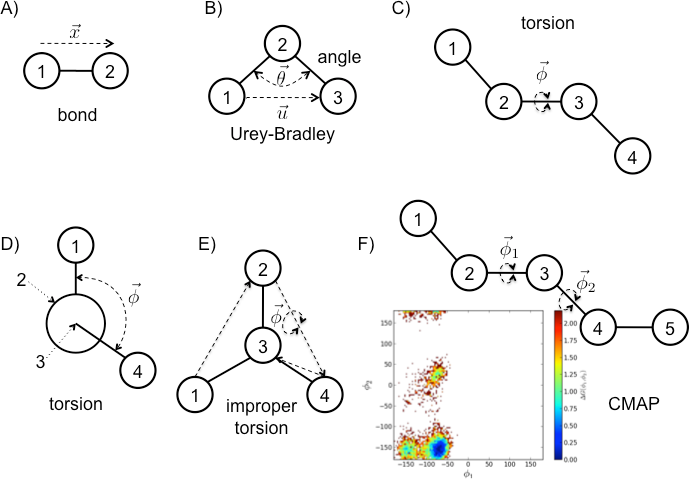
\includegraphics[width=6.5in,height=4.7in]{Parameters.png}
   \caption[Schematics shown for various parameters present in typical force
            fields.]
           {Schematics shown for various parameters present in typical force
            fields. A) is a bond parameter, B) shows the valence angle parameter
            and the Urey-Bradley parameter where $\vec{u}$ is the shown
            distance, C) depicts a torsion, D) depicts the same torsion using a
            Newman projection, E) depicts an improper torsion, and F) depicts
            two coupled torsions alongside a typical free energy map of two
            torsions that CMAP parameters attempt to fit to.}
   \label{fig1:Parameters}
\end{figure}

\subsection{The Amber Force Field}

The Amber force field is a popular family of force fields designed to treat
large biomolecules such as proteins, DNA, and RNA. This section will focus on
the functional form and implementation of the Amber force fields
\cite{Cornell_JAmChemSoc_1995_v117_p5179, Duan03, Hornak_Proteins_2006_v65_p712}
in the supporting Amber programs. \cite{Case_JComputChem_2005_v26_p1668}

\subsubsection{Functional Form}

The functional form of the Amber force fields is typically presented as in Eq.
\ref{eq1:AmberFF}, \cite{Cornell_JAmChemSoc_1995_v117_p5179} although this is an
incomplete specification. A more rigorous definition is presented in Eq.
\ref{eq1:AmberFF2}, taking into account the proper exclusion of non-bonded terms
between bonded atoms.

\begin{align}
   U(q) & = \sum _ {\text{bonds}} K_r ( r - r_{eq}) ^ 2 + \sum _ {\text{angles}}
          K_{\theta} ( \theta - \theta _ {eq} ) ^ 2 \nonumber \\
      & + \sum _ {\text{torsions}} \frac {V_n} 2 \left [ 1 + \cos (n \phi -
          \gamma) \right ] + \frac 1 2 \sum _ {i} \sum _ {j} \left [ \frac
          {A_{i,j}} {R_{i,j} ^ {12}} - \frac {B_{i,j}} {R_{i,j} ^ 6} + k_{elec}
          \frac {q_i q_j} {\epsilon R_{i, j}} \right ]
   \label{eq1:AmberFF}
\end{align}

\begin{align}
    & \sum _ {\text{bonds}} K_r ( r - r_{eq}) ^ 2 + \sum _ {\text{angles}} +
          K_{\theta} ( \theta - \theta _ {eq} ) ^ 2 \nonumber + \\
   U(q) = & \sum _ {\text{torsions}} \frac {V_n} 2 \left [ 1 + \cos (n \phi -
      \gamma) \right ] + \frac 1 2 \sum _ {i} \sum _ {j \in l_{1-4,i}} \left [
      \frac {A_{i,j}} {2.0 R_{i,j} ^ {12}} - \frac {B_{i,j}} {2.0 R_{i,j} ^ 6} +
      \frac {q_i q_j} {1.2 \epsilon R _{i,j}} \right ] +
      \label{eq1:AmberFF2} \\
    & \frac 1 2 \sum _ {i} \sum _ {j \notin l_{excl,i}} \left [ \frac {A_{i,j}}
      {R_{i,j} ^ {12}} - \frac {B_{i,j}} {R_{i,j} ^ 6} + k_{elec} \frac {q_i
      q_j} {\epsilon R_{i, j}} \right ] \nonumber
\end{align}

Amber employs a simple harmonic potential to model angles and bonds to
completely describe the interactions between atoms separated by one and two
bonds---\ie no electrostatic or Lennard-Jones potentials are calculated between
pairs of atoms connected by a bond or angle. Torsions are treated with a
truncated Fourier series expansion, typically using integral values for the
periodicity ($n$ in Eqs. \ref{eq1:AmberFF} and \ref{eq1:AmberFF2}). Therefore,
the sum over torsions in Eqs. \ref{eq1:AmberFF} and \ref{eq1:AmberFF2} is a sum
over all individual torsion terms for each distinct torsion. Improper torsions
are modeled the same way as `proper' torsions with only a single term designed
to maintain their planar geometry.

The non-bonded interactions are composed of a Lennard-Jones term (the third form
of Eq. \ref{eq1:LennardJones}) and electrostatic term calculated between all
atom pairs that are not excluded from the computation. The non-bonded exclusion
list---$l_{excl,i}$ for atom $i$ in Eq. \ref{eq1:AmberFF2}---is composed all
atoms separated by one, two, and three bonds (\ie that form bonds, angles, or
torsions with atom $i$). Finally, the LJ interactions between all atoms
separated by three bonds are scaled by $1/2$ and the electrostatic interactions
between those atom pairs are scaled by $1/1.2$. In Eq. \ref{eq1:AmberFF2},
$l_{1-4,i}$ represents the list of atoms related to atom $i$ like atoms 1 and
4 in Fig. \ref{fig1:Parameters}C.

\subsubsection{Implementation}

This section will describe how the Amber family of force fields is implemented
in the Amber program suite. It is important to note that the Amber force field
is not unique---there are many variants, each with a different name.
\cite{Cornell_JAmChemSoc_1995_v117_p5179, Wang_JComputChem_2000_v21_p1049,
Duan03, Wang_JComputChem_2004_v25_p1157, Hornak_Proteins_2006_v65_p712,
Zgarbova_JChemTheoryComput_2011_v7_p2886} All information necessary to fully
describe a molecular system with the Amber force field is contained in two
files---the parameter-topology file (\emph{prmtop}) and the coordinate file. The
prmtop file---fully described in Appendix \ref{appendixB}---contains all of the
information regarding the bonded network and the necessary parameters for
evaluating Eq. \ref{eq1:AmberFF2}. The coordinate file contains the Cartesian
coordinates and velocities for each atom in the system described by the prmtop
file.

The prmtop file is generated by the \emph{tleap} program by matching the
parameters from a database to the assigned `atom types' of the input structure.
Atom types are descriptors of individual atoms that specifies the properties and
typical chemical structure of bonds involving that atom. Each atom type, $i$,
has a predetermined set of atom parameters---an atomic mass, a LJ radius $r_i$,
and a LJ well-depth $\varepsilon_i$. The pairwise $R_{min,i,j}$ in Eq.
\ref{eq1:LennardJones} of atom types $i$ and $j$ is the sum $r_i + r_j$. The
combined well depth $\varepsilon_{i,j}$ is the geometric mean of the individual
well depths ($\sqrt {\varepsilon_i \varepsilon_j}$). These are the so-called
\emph{combining rules} employed by \emph{tleap} when parametrizing a molecule
with an Amber force field.

The Amber parameter databases store a list of all recognized atom types as well
as the bond, angle, and torsion parameters between the various bonded
arrangements of the available atom types. For instance, each pair of atom types
that could form a bond (\eg two aromatic carbons or an aromatic carbon and an
aromatic hydrogen) has an equilibrium bond length and bond force constant
associated with it. Also stored in these parameter databases are the equilibrium
angle displacements with corresponding force constants and torsion parameters
(periodicities, barrier heights, and phase shifts for each term of every
torsion).


%------------------------------------------------------------------------------%

% Includes appendices called into the appendix file(check the comments regarding
% editing your appendix in that file)
% The Editorial Office Requirements for the Table of Contents cause a significant problem 
%in Latex if there is only one Appendix. The Appendix is no longer labeled "A" in the TOC
%but has the word "APPENDIX" placed in front of the title of the Appendix. This can be done
%without issue IF nothing needs to be numbered by LaTeX in the Appendix. Unfortunately, most of the time
%something needs to be numbered in that single Appendix. For this reason we have included the IFTHENELSE switch
%found in this document and at the beginning of AppendixA. We assume that if you have any appendices, that you have more than one.
%So the default setting is noa = 2 (number of appendices = 2). Note: you don't need the actual number of appendices here
%1 or 2 are the only relevant numbers. You just make sure to input the Appendices you do have in this file.
%
%If, however, you DO only have one appendix change the line:
%
%\setcounter{noa}{2} to
%
%\setcounter{noa}{1}
%
%And comment (or delete) all of the input{AppendixB} commands except the first one.
%Then open the AppendixA.tex file and continue there.

%you can add/substract individual appendices through by using the /include{appendix'X'}
% and creating/deleting the appropriate files
\appendix %
\clearpage%
\newcounter{noa} % noa= no. of appendices ... set to 1 for 1 and more otherwise.
\setcounter{noa}{3} % ........................... CHANGE VALUE ONLY HERE
\ifthenelse{\value{noa} = 1}
%...................then
{}
%...................else
{\addtocontents{toc}{\protect\addvspace{10pt}\protect\noindent \protect APPENDIX}}
%...................
% Conditional branch in the case where there is only one appendix (noa = 1) or
% more than one
\ifthenelse{\value{noa} = 1}
%...................then
{\chapter*{APPENDIX: THIS IS THE FIRST APPENDIX}
\addcontentsline{toc}{chapter}{APPENDIX: THIS IS THE FIRST APPENDIX}
\chaptermark{Appendix}
\markboth{Appendix}{Appendix}
\setcounter{chapter}{1}}
%...................else
{\chapter{NUMERICAL INTEGRATION IN CLASSICAL MOLECULAR DYNAMICS}}
%...................
\label{appendixA}

\section{Lagrangian and Hamiltonian Formulations}

The \emph{Lagrangian} and \emph{Hamiltonian} formulations of classical
mechanics---shown in Eqs. \ref{eqA:Lagrangian} and \ref{eqA:Hamiltonian},
respectively---offer a more convenient formalism than the more popularly known
equations derived by Newton. \cite{CorbenClassicalMechanics} While Newton's
equations apply in three-dimensional Cartesian space, they are not generally
applicable to other coordinate systems (\eg polar and spherical-polar
coordinates) that may be a more natural way to express certain problems. For
instance, polar coordinates more naturally describe the mechanics of orbiting
bodies than standard Euclidean space.

\textbf{Lagrangian Equation.} The Lagrangian function, $L = K - V$, where $K$ is
the kinetic energy and $V$ is the potential energy, satisfies the Lagrangian
equation (Eq.  \ref{eqA:Lagrangian}) for $m$ generalized coordinates ($q_m$).
The advantage of Eq. \ref{eqA:Lagrangian} is that it is derived without any
assumption of a specific coordinate system for $q_m$. Generalized velocities are
the first time-derivative of the generalized coordinates, $\dot q_m$. These
generalized velocities are used to define the kinetic energy in the familiar
form $K = 1/2 \dot q_m ^ 2$.

Another advantage to the Lagrangian formulation of classical mechanics is that
the equations are still valid when subject to constraints on the dynamics of the
system (as long as there are fewer constraints than particles).
\cite{CorbenClassicalMechanics} This property is crucial for carrying out
constrained dynamics, such as those simulations employing the commonly-used
SHAKE, \cite{Ryckaert_JComputPhys_1977_v23_p327} RATTLE, \cite{Andersen1983} or
SETTLE \cite{Miyamoto_JComputChem_1992_v13_p952} algorithms, to name a few.

\begin{equation}
   \frac d {dt} \frac {\partial L} {\partial \dot q_m} - \frac {\partial L}
         {\partial q_m} = 0
   \label{eqA:Lagrangian}
\end{equation}
$L$ in Eq. \ref{eqA:Lagrangian} is the Lagrangian function mentioned above,
$q_m$ are the generalized coordinates of every particle in the system, and $\dot
q_m$ are the set of corresponding generalized velocities. When applying Eq.
\ref{eqA:Lagrangian} to a system in the standard Cartesian coordinates without
constraints, the familiar form of Newton's equations are recovered.
\cite{CorbenClassicalMechanics}

\textbf{Hamiltonian Equation.} The Hamiltonian formulation of classical
mechanics builds on the strengths of the Lagrangian formulation and provides a
deeper insight into the physical behavior of classical systems. Unlike the
Lagrangian, the Hamiltonian is defined as the total energy of the system: $H = K
+ V$. The Lagrangian of the system, $L = K - V$, plays an important part in
Hamilton's formulation. The degrees of freedom in Hamilton's equation (Eq.
\ref{eqA:Hamiltonian}) are the generalized coordinates $q_m$ as defined in the
Lagrangian, and their conjugate momenta, $p_m$. The generalized coordinates and
momenta are said to be canonically conjugate because they obey the relationship
given in Eq. \ref{eqA:Hamiltonian}. \cite{CorbenClassicalMechanics}

\begin{align}
   q_m & = \frac {\partial H} {\partial p_m} \nonumber \\
   p_m & = - \frac {\partial H} {\partial q_m}
   \label{eqA:Hamiltonian}
\end{align}

Now that a convenient formulation of the laws of classical dynamics are known, I
will shift the discussion toward techniques by which these equations are used to
integrate these second-order differential equations in typical molecular
dynamics simulations.

\section{Numerical Integration by Finite Difference Methods}

The equations of motion are second-order differential equations with respect to
the particle coordinates, since the force is proportional to the second
time-derivative (\ie the acceleration) of those particles. Due to the typical
size and complexity of the systems and their potentials studied in computational
chemistry, MD simulations require numerical integration of the second-order
differential equations of motion. In this section, I will describe two common
approaches to iteratively integrating Eqs. \ref{eqA:Lagrangian} and
\ref{eqA:Hamiltonian}---so-called \emph{predictor-corrector} methods and the
Verlet family of integrators.

\subsection{Predictor-corrector}

The predictor-corrector integrators are based on a simple Taylor-series
expansion of the coordinates. Knowing that the velocity and acceleration are the
first- and second-time derivatives of the particle positions, respectively, the
Taylor expansions of each of these quantities are given below.
\begin{align}
   \vec{r}_p (t_0 + \delta t) & = \vec{r}(t_0) + \delta t \, \vec{v}(t_0) +
         \delta t^2 \, \frac 1 2 \vec{a}(t_0) + \delta t^3 \, \frac 1 6 \frac
         {d^3\vec{r}(t)} {dt^3} + ... \nonumber \\
   \vec{v}_p (t_0 + \delta t) & = \vec{v}(t_0) + \delta t \, a(t) + \frac 1 2 
         \delta t^2 \, \frac {d^3\vec{r}(t)} {dt^3} + ...
   \label{eqA:Predictor} \\
   \vec{a}_p (t_0 + \delta t) & = \vec{a}(t_0) + \delta t \, \frac
         {d^3\vec{r}(t)} {dt^3} + ... \nonumber
\end{align}
The subscript $p$ in these equations emphasizes that these are the
\emph{predicted} quantities of the positions, velocities, and accelerations at
time $t_0 + \delta t$ based on the known values at time $t_0$.

It is convenient to truncate the Taylor series in Eqs. \ref{eqA:Predictor} after
the acceleration term since the acceleration at time $t_0$ can be easily
calculated from the gradient of the potential energy function. Higher order
terms are difficult to compute, and contribute a significantly smaller amount as
the time step, $\delta t$, decreases. However, by truncating the Taylor
expansion we used an approximation that will introduce systematic error of our
predicted values calculated by Eqs. \ref{eqA:Predictor} compared to their
\emph{true} values. There is a way of approximating the magnitude of the
deviation of the predicted values from Eqs. \ref{eqA:Predictor}, however, that
will allow a correction to be applied to the integrated values.

As a reminder, the gradient of the potential was used to calculate the
forces---and therefore the acceleration---on each particle when making the
initial integration step from $t_0$. The acceleration may be calculated again
using the gradient of the potential at the predicted conformations:
\begin{equation}
   \bigtriangledown V\left[\vec{r}_p(t_0 + \delta t)\right] = m \vec{a}^{\prime}
   \label{eqA:ErrorCorrection}
\end{equation}
Since systematic error has been introduced by truncating the expansion in Eqs.
\ref{eqA:Predictor}, $\vec{a}^{\prime}$ from Eq. \ref{eqA:ErrorCorrection} and
$\vec{a}_p(t_0 + \delta t)$ from Eq. \ref{eqA:Predictor} will differ. The
magnitude of this difference can be used to correct the predicted values
according to Eqs. \ref{eqA:Corrector}.

\begin{align}
   \vec{r}_c(t + \delta t) & = \vec{r}_p(t + \delta t) + c_0 \Delta \vec{a}(t +
         \delta t) \nonumber \\
   \vec{v}_c(t + \delta t) & = \vec{v}_p(t + \delta t) + c_1 \Delta \vec{a}(t +
         \delta t)
   \label{eqA:Corrector} \\
   \vec{a}_c(t + \delta t) & = \vec{a}_p(t + \delta t) + c_2 \Delta \vec{a}(t +
         \delta t) \nonumber
\end{align}
where the subscripts indicate the relationship between the \emph{c}orrected and
\emph{p}redicted quantities, and the coefficients $c_0$, $c_1$, and $c_2$ are
parametrized to maximize performance, \cite{Gear1966, Gear1971} and have the
appropriate units to satisfy each equation. \cite{Allen_Tildesley} The corrector
process can be iterated until the desired level of agreement between the
predicted and corrected values is reached.

While the predictor-corrector algorithm allows long time steps to be taken by
fixing the resulting systematic error, the corrector step requires a full force
evaluation of the system at a set of coordinates, which is the most
time-consuming portion of the calculation. As a result, the corrector step is
computationally demanding, and predictor-corrector methods have been replaced by
other integration schemes in standard practice.

\subsection{Verlet Integrators}

Among the most popular types of integrators in common use today are based on the
\emph{Verlet} algorithms. The Verlet algorithm, developed in
\citeyear{Verlet_PhysRev_1967_v159_p98} by
\citeauthor{Verlet_PhysRev_1967_v159_p98}, utilizes a Taylor series expansion of
the particle coordinates about time $t_0$. The key to the Verlet approach is to
use both the forward and reverse time steps, as shown in Eqs.
\ref{eqA:PositionExpansion}. \cite{Allen_Tildesley}

\begin{align}
   \vec{r}(t_0 + \delta t) = r(t_0) + \delta t \, \vec{v}(t_0) + \frac 1 2
         \delta t^2 \, \vec{a}(t_0) + ... \nonumber \\
   \vec{r}(t_0 - \delta t) = r(t_0) - \delta t \, \vec{v}(t_0) + \frac 1 2
         \delta t^2 \, \vec{a}(t_0) - ...
   \label{eqA:PositionExpansion}
\end{align}

Combining Eqs. \ref{eqA:PositionExpansion} gives
\begin{equation}
   \vec{r}(t_0 + \delta t) = 2 \vec{r}(t_0) + \delta t^2 \, \vec{a}(t_0) -
         \vec{r}(t_0 - \delta t)
   \label{eqA:Verlet}
\end{equation}
where the velocities have been eliminated from the expression and are therefore
unnecessary when integrating the equations of motion. Furthermore, like the
velocities, the $\delta t^3$ term also cancels, so the Verlet algorithm is not
only time-reversible given its symmetry around $t_0$ but also accurate to fourth
order in the time step. The velocities are still useful, however, to compute the
total kinetic energy and related properties, such as the instantaneous
temperature. When necessary, velocities can be approximated as the average
velocity over the time period from $t_0-\delta t$ to $t_0+\delta t$.

Performing MD using the Verlet algorithm requires storing the current positions,
`old' positions at time $t_0-\delta t$, and the accelerations at time $t_0$---a
modest cost given the accuracy of the integration scheme. However, the use of
Eq. \ref{eqA:Verlet} introduces an issue of numerical precision, since
$\vec{r}(t_0)$ and $\vec{r}(t_0 - \delta t)$ are potentially large values, while
$\delta t^2 \, \vec{a}(t_0)$ is typically quite small since the time step is
small. Since real numbers can be stored only to a limited precision, accuracy is
potentially lost when a small number is added to a difference of large numbers.
\cite{Allen_Tildesley} To address this issue and improve the way in which
velocities are handled, the leap-frog and velocity Verlet methods are discussed
below.

\textbf{Velocity Verlet.} In \citeyear{Swope_JChemPhys_1982_v76_p637},
\citeauthor{Swope_JChemPhys_1982_v76_p637} developed a variant of the Verlet
algorithm that sidesteps the potential roundoff errors and naturally stores
positions, velocities, and accelerations at the same time. A Taylor series
expansion is again used to propagate the positions, but only the $t_0+\delta t$
step is used, resulting in Eq. \ref{eqA:VelVerletPositions}.
\begin{equation}
   \vec{r}(t_0 + \delta t) = \vec{r}(t_0) + \delta t \, \vec{v}(t_0) + \frac 1 2
         \delta t^2 \, \vec{a}(t_0)
   \label{eqA:VelVerletPositions}
\end{equation}
The accelerations of the particles are computed from their positions at time
$t_0 + \delta t$, and are used to compute the velocities. To increase the
accuracy of the computed velocities, the velocity integration is divided into
two half-timesteps, shown in Eqs. \ref{eqA:VelVerletVelocities}. In this case,
the accuracy to $\delta t^4$ in the positions obtained by the Verlet algorithm
is sacrificed for improved numerical precision for finite-precision computers
and a more accurate treatment of system velocities.

\begin{align}
   \vec{v}\left(t_0 + \frac 1 2 \delta t\right) = \vec{v}(t_0) + \frac 1 2
         \delta t \, \vec{a}(t_0) \nonumber \\
   \vec{v}(t_0 + \delta t) = \vec{v}\left(t_0 + \frac 1 2 \delta t\right) +
         \frac 1 2 \delta t \, \vec{a}(t_0 + \delta t) \nonumber \\
   \vec{v}(t_0 + \delta t) = \vec{v}(t) + \frac 1 2 \delta t \left[ \vec{a}(t) +
         \vec{a}(t + \delta t) \right]
   \label{eqA:VelVerletVelocities}
\end{align}

The \emph{NAB} and \emph{mdgx} programs of the AmberTools 12 program suite (and
earlier versions, where available), utilize the velocity Verlet algorithm for
dynamics.

\textbf{Leap-frog.} A common integrator used in MD simulations is the
\emph{leap-frog} method, so-called because the computed velocities `leap' over
the computed coordinates in a manner that will be explained shortly. The main
dynamics engines in the Amber 12 program suite---pmemd and sander---use the
leap-frog integrator.

While similar to the velocity Verlet approach, the leap-frog algorithm computes
positions and accelerations of particles at integral time steps, but
computes velocities at half-integral time steps according to Eqs.
\ref{eqA:LeapFrog}.

\begin{align}
   \vec{r}(t_0 + \delta t) = \vec{r}(t_0) + \delta t \, \vec{v}\left(t_0 + \frac
         1 2 \delta t \right) \nonumber \\
   \vec{v}\left(t_0 + \frac 1 2 \delta t\right) = \vec{v}\left(t_0 - \frac 1 2
         \delta t \right) + \delta t \, \vec{a}(t_0)
   \label{eqA:LeapFrog}
\end{align}

If the velocities are required at time $t_0$, they can be estimated as the
average velocities between times $t_0 - 1/2\delta t$ and $t_0 + 1/2 \delta t$,
which is significantly more accurate than the approximation in Verlet's original
algorithm. Like the velocity Verlet algorithm, leap-frog integration sacrifices
the 4th-order accuracy in integrated positions to alleviate the aforementioned
precision and velocity issues. \cite{Allen_Tildesley}

\chapter{AMBER Parameter-Topology File Format}%
\label{appendixB}

This appendix details the Parameter-Topology file format used extensively by the
AMBER software suite for biomolecular simulation and analysis, referred to as
the \emph{prmtop} file for short. The format specification of the AMBER topology
file was written initially over a decade ago and posted on
http://ambermd.org/formats.html. I have recently expanded that document to
account for the drastic change to the file format that occurred with the 2004
release of Amber 7. The pre-Amber 7 format (\emph{old format}) is described more
briefly afterwards, although each section provided in the original format
contains exactly the same information as the newer version.

This appendix also details the format changes and additions introduced by
\emph{chamber}---the program that translates a CHARMM parameter file (PSF) into
a topology file that can be used with the \emph{sander} and \emph{pmemd}
programs in AMBER.

This appendix draws from the information on http://ambermd.org/formats.html that
was added by both me and others, as well as the experience I gleaned while
writing the ParmEd program and working with the various codes in AMBER.

As a warning, the prmtop file is a result of bookkeeping that becomes
increasingly complex as the system size increases. Therefore, hand-editing the
topology file for all but the smallest systems is discouraged---a program or
script should be written to automate the procedure.

\section{Layout}

The first line of the Amber topology file is the version string. An example is
shown below in which {\tt XX} is replaced by the actual date and time.
\begin{verbatim}
%VERSION  VERSION_STAMP = V0001.000  DATE = XX/XX/XX  XX:XX:XX
\end{verbatim}

The topology format is divided into several sections in a way that is designed
to be parsed easily using simple Fortran code. A consequence of this is that it
is difficult for parsers written in other languages (\eg C, C++, Python, etc.)
to strictly adhere to the standard. These parsers should try, however, to
support as much of the standard as possible.

\begin{verbatim}
%FLAG SECTION
%COMMENT an arbitrary number of optional comments may be put here
%FORMAT(<FORTRAN FORMAT>)
... data formatted according to <FORTRAN FORMAT>
\end{verbatim}

All names (\eg atom names, atom type names, and residue names) are limited to
4 characters and are printed in fields of width \emph{exactly} 4 characters
wide, left-justified. This means that names might not be space-delimited if any
of the names have 4 characters.

\paragraph{Requirements for prmtop parsers}

Parsers, regardless of the language they are written in, should conform to a
list of attributes to maximize the likelihood that they are parsed correctly.

\begin{itemize}
   \item Parsers should expect that some 4-character fields (\eg atom or residue
         names) may have some names that have 4 characters and therefore might
         not be whitespace-delimited.
   \item Parsers should not expect {\tt SECTION}s in the prmtop to be in any
         particular order.
   \item Parsers should not expect or require {\tt \%COMMENT} lines to exist,
         but should properly parse the file if any number of {\tt \%COMMENT}
         lines appear as indicated above
   \item The topology file may be assumed to have been generated `correctly' by
         \emph{tleap} or some other credible source. No graceful error checking
         is required.
\end{itemize}

\paragraph{Requirements for modifying {\tt SECTION}s}

To minimize the impact of prmtop changes to existing, third-party parsers, the
following conventions should be followed.

\begin{itemize}
   \item Any new {\tt SECTION} should be added to the end of the topology file to
         avoid conflicts with order-dependent parsers.
   \item The {\tt <FORTRAN FORMAT>} should be as simple as possible (and avoid
         adding new formats) to maintain simplicity for non-Fortran parsers.
   \item Avoid modifying if possible. Consider if this new section or change is
         truly necessary \emph{and} belongs in the prmtop.
\end{itemize}

\section{List of {\tt SECTION}s}

\subsection*{TITLE}

This section contains the title of the topology file on one line (up to 80
characters). While the title serves a primarily cosmetic purpose, this section
must be present.

\noindent {\tt \%FORMAT(20a4)}

\subsection*{POINTERS}

This section contains the information about how many parameters are present in
all of the sections. There are 31 or 32 integer pointers (NCOPY might not be
present). The format and names of all of the pointers are listed below, followed
by a description of each pointer.

\vspace{8pt}
\hline
\vspace{4pt}

\begin{verbatim}
%FLAG POINTERS
%FORMAT(10I8)
NATOM  NTYPES NBONH  MBONA  NTHETH MTHETA NPHIH  MPHIA  NHPARM NPARM  
NNB    NRES   NBONA  NTHETA NPHIA  NUMBND NUMANG NPTRA  NATYP  NPHB   
IFPERT NBPER  NGPER  NDPER  MBPER  MGPER  MDPER  IFBOX  NMXRS  IFCAP  
NUMEXTRA NCOPY 
\end{verbatim}

\vspace{4pt}
\hline
\vspace{8pt}

\begin{description}
   \item[NATOM] Number of atoms
   \item[NTYPES] Number of distinct Lennard-Jones atom types
   \item[NBONH] Number of bonds containing Hydrogen
   \item[MBONA] Number of bonds not containing Hydrogen
   \item[NTHETH] Number of angles containing Hydrogen
   \item[MTHETA] Number of angles not containing Hydrogen
   \item[NPHIH] Number of torsions containing Hydrogen
   \item[MPHIA] Number of torsions not containing Hydrogen
   \item[NHPARM] Not currently used for anything
   \item[NPARM] Used to determine if this is a LES-compatible prmtop
   \item[NNB] Number of excluded atoms (length of total exclusion list)
   \item[NRES] Number of residues
   \item[NBONA] MBONA + number of constraint bonds \footnote{AMBER codes no
         longer support constraints in the topology
         file.}\addtocounter{footnote}{-1}\addtocounter{Hfootnote}{-1}
   \item[NTHETA] MTHETA + number of constraint angles
         \footnotemark\addtocounter{footnote}{-1}\addtocounter{Hfootnote}{-1}
   \item[NPHIA] MPHIA + number of constraint torsions \footnotemark
   \item[NUMBND] Number of unique bond types
   \item[NUMANG] Number of unique angle types
   \item[NPTRA] Number of unique torsion types
   \item[NATYP] Number of SOLTY terms. Currently unused.
   \item[NPHB] Number of distinct 10-12 hydrogen bond pair types
      \footnote{Modern AMBER force fields do not use a 10-12 potential}
   \item[IFPERT] Set to 1 if topology contains residue perturbation information.
      \footnote{No AMBER codes support perturbed topologies anymore}
      \addtocounter{footnote}{-1}\addtocounter{Hfootnote}{-1}
   \item[NBPER] Number of perturbed bonds \footnotemark
      \addtocounter{footnote}{-1} \addtocounter{Hfootnote}{-1}
   \item[NGPER] Number of perturbed angles \footnotemark
      \addtocounter{footnote}{-1} \addtocounter{Hfootnote}{-1}
   \item[NDPER] Number of perturbed torsions \footnotemark
      \addtocounter{footnote}{-1} \addtocounter{Hfootnote}{-1}
   \item[MBPER] Number of bonds in which both atoms are being perturbed
      \footmarknote \addtocounter{footnote}{-1} \addtocounter{Hfootnote}{-1}
   \item[MGPER] Number of angles in which all 3 atoms are being perturbed
      \footmarknote \addtocounter{footnote}{-1} \addtocounter{Hfootnote}{-1}
   \item[MDPER] Number of torsions in which all 4 atoms are being perturbed
      \footnotemark
   \item[IFBOX] Flag indicating whether a periodic box is present. Values can be
      0 (no box), 1 (orthorhombic box) or 2 (truncated octahedron)
   \item[NMXRS] Number of atoms in the largest residue
   \item[IFCAP] Set to 1 if a solvent CAP is being used
   \item[NUMEXTRA] Number of extra points in the topology file
   \item[NCOPY] Number of PIMD slices or number of beads
\end{description}

\subsection*{ATOM\_NAME}

This section contains the atom name for every atom in the prmtop.

\noindent {\tt \%FORMAT(20a4)}
\noindent There are {\tt NATOM} 4-character strings in this section.

\subsection*{CHARGE}

This section contains the charge for every atom in the prmtop. Charges are
multiplied by 18.2223 ($\sqrt{k_{ele}}$ where $k_{ele}$ is the electrostatic
constant in $kcal\, \AA\, mol^{-1}\, q^{-2}$, where $q$ is the charge of an
electron).

\noindent {\tt \%FORMAT(5E16.8)}

\noindent There are {\tt NATOM} floating point numbers in this section.

\subsection*{ATOMIC\_NUMBER}

This section contains the atomic number of every atom in the prmtop. This
section was first introduced in AmberTools 12. \cite{AMBER12}

\noindent {\tt \%FORMAT(10I8)}

\noindent There are {\tt NATOM} integers in this section.

\subsection*{MASS}

This section contains the atomic mass of every atom in $g\, mol^{-1}$.

\noindent {\tt \%FORMAT(5E16.8)}

\noindent There are {\tt NATOM} floating point numbers in this section.

\subsection*{ATOM\_TYPE\_INDEX}

This section contains the Lennard-Jones atom type index. The Lennard-Jones
potential contains parameters for every pair of atoms in the system. To minimize
the memory requirements of storing {\tt NATOM} $\times$ {\tt NATOM}
\footnote{Only half this number would be required, since $a_{i,j} \equiv
a_{j,i}$} Lennard-Jones A-coefficients and B-coefficients, all atoms with the
same $\sigma$ and $\varepsilon$ parameters are assigned to the same type
(regardless of whether they have the same {\tt AMBER\_ATOM\_TYPE}). This
significantly reduces the number of LJ coefficients which must be stored, but
introduced the requirement for bookkeeping sections of the topology file to keep
track of what the LJ type index was for each atom.

This section is used to compute a pointer into the {\tt NONBONDED\_PARM\_INDEX}
section, which itself is a pointer into the {\tt LENNARD\_JONES\_ACOEF} and {\tt
LENNARD\_JONES\_BCOEF} sections (see below).

\noindent {\tt \%FORMAT(10I8)}

\noindent There are {\tt NATOM} integers in this section.

\subsection*{NUMBER\_EXCLUDED\_ATOMS}

This section contains the number of atoms that need to be excluded from the
non-bonded calculation loop for atom $i$ because $i$ is involved in a bond,
angle, or torsion with those atoms. Each atom in the prmtop has a list of
excluded atoms that is a subset of the list in {\tt EXCLUDED\_ATOMS\_LIST} (see
below). The $i$th value in this section indicates how many elements of {\tt
EXCLUDED\_ATOMS\_LIST} belong to atom $i$.

For instance, if the first two elements of this array is 5 and 3, then elements
1 to 5 in {\tt EXCLUDED\_ATOMS\_LIST} are the exclusions for atom 1 and elements
6 to 8 in {\tt EXCLUDED\_ATOMS\_LIST} are the exclusions for atom 2. Each
exclusion is listed only once in the topology file, and is given to the atom
with the smaller index. That is, if atoms 1 and 2 are bonded, then atom 2 is in
the exclusion list for atom 1, but atom 1 is \emph{not} in the exclusion list
for atom 2. If an atom has no excluded atoms (either because it is a monoatomic
ion or all atoms it forms a bonded interaction with have a smaller index), then
it is given a value of 1 in this list which corresponds to an exclusion with (a
non-existent) atom 0 in {\tt EXCLUDED\_ATOMS\_LIST}.

The exclusion rules for extra points are more complicated. When determining
exclusions, it is considered an `extension' of the atom it is connected (bonded)
to. Therefore, extra points are excluded not only from the atom they are
connected to, but also from every atom that its parent atom is excluded from.

\emph{NOTE}: The non-bonded interaction code in \emph{sander} and \emph{pmemd}
currently (as of Amber 12) recalculates the exclusion lists for simulations of
systems with periodic boundary conditions, so this section is effectively
ignored. The GB code uses the exclusion list in the topology file.

\noindent {\tt \%FORMAT(10I8)}

\noindent There are {\tt NATOM} integers in this section.

\subsection*{NONBONDED\_PARM\_INDEX}

This section contains the pointers for each pair of LJ atom types into the {\tt
LENNARD\_JONES\_ACOEF} and {\tt LENNARD\_JONES\_BCOEF} arrays (see below). The
pointer for an atom pair in this array is calculated from the LJ atom type index
of the two atoms (see {\tt ATOM\_TYPE\_INDEX} above).

The index for two atoms $i$ and $j$ into the {\tt LENNARD\_JONES\_ACOEF} and
{\tt LENNARD\_JONES\_BCOEF} arrays is calculated as 
\begin{equation}
   index = {\tt NONBONDED\_PARM\_INDEX} \left [ {\tt NTYPES} \times \left ( {\tt
      ATOM\_TYPE\_INDEX}(i) - 1 \right ) + {\tt ATOM\_TYPE\_INDEX}(j) \right ]
   \label{eqB:ParmIndex}
\end{equation}

Note, each atom pair can interact with either the standard 12-6 LJ potential
\emph{or} via a 12-10 hydrogen bond potential. If $index$ in Eq.
\ref{eqB:ParmIndex} is negative, then it is an index into {\tt HBOND\_ACOEF} and
{\tt HBOND\_BCOEF} instead (see below).

\noindent {\tt \%FORMAT(10I8)}

\noindent There are ${\tt NTYPES} \times {\tt NTYPES}$ integers in this section.

\subsection*{RESIDUE\_LABEL}

This section contains the residue name for every residue in the prmtop. Residue
names are limited to 4 letters, and might not be whitespace-delimited if any
residues have 4-letter names.

\noindent {\tt \%FORMAT(20a4)}

\noindent There are {\tt NRES} 4-character strings in this section.

\subsection*{RESIDUE\_POINTER}

This section lists the first atom in each residue.

\noindent {\tt \%FORMAT(10i8)}

\noindent There are {\tt NRES} integers in this section.

\subsection*{BOND\_FORCE\_CONSTANT}

Bond energies are calculated according to the equation
\begin{equation}
   E_{bond} = \frac 1 2 k \left ( \vec{r} - \vec{r}_{eq} \right ) ^ 2
   \label{eqB:Bond}
\end{equation}

This section lists all of the bond force constants ($k$ in Eq. \ref{eqB:Bond})
in units $kcal\, mol^{-1}\, \AA^{-2}$ for each unique bond type. Each bond in
{\tt BONDS\_INC\_HYDROGEN} and {\tt BONDS\_WITHOUT\_HYDROGEN} (see below)
contains an index into this array.

\noindent {\tt \%FORMAT(5E16.8)}

\noindent There are {\tt NUMBND} floating point numbers in this section.

\subsection*{BOND\_EQUIL\_VALUE}

This section lists all of the bond equilibrium distances ($\vec{r}_{eq}$ in Eq.
\ref{eqB:Bond}) in units of \AA for each unique bond type. This list is indexed
the same way as {\tt BOND\_FORCE\_CONSTANT}.

\noindent {\tt \%FORMAT(5E16.8)}

\noindent There are {\tt NUMBND} floating point numbers in this section.

\subsection*{ANGLE\_FORCE\_CONSTANT}

Angle energies are calculated according to the equation
\begin{equation}
   E_{angle} = \frac 1 2 k_{\theta} \left ( \theta - \theta _ {eq} \right ) ^ 2
   \label{eqB:Angle}
\end{equation}

This section lists all of the angle force constants ($k_{\theta}$ in Eq.
\ref{eqB:Angle}) in units of $kcal\, mol^{-1}\, rad^2$ for each unique angle
type. Each angle in {\tt ANGLES\_INC\_HYDROGEN} and {\tt
ANGLES\_WITHOUT\_HYDROGEN} contains an index into this (and the next) array.

\noindent {\tt \%FORMAT(5E16.8)}

\noindent There are {\tt NUMANG} floating point numbers in this section.

\subsection*{ANGLE\_EQUIL\_VALUE}

This section contains all of the angle equilibrium angles ($\theta_{eq}$ in Eq.
\ref{eqB:Angle}) in radians.  \emph{NOTE:} the AMBER parameter files list
equilibrium angles in degrees and are converted to radians in \emph{tleap}. This
list is indexed the same way as {\tt ANGLE\_FORCE\_CONSTANT}.

\noindent {\tt \%FORMAT(5E16.8)}

\noindent There are {\tt NUMBND} floating point numbers in this section.

\subsection*{DIHEDRAL\_FORCE\_CONSTANT}

Torsion energies are calculated for each term according to the equation
\begin{equation}
   E_{torsion} = k_{tor} \cos \left ( n \phi + \psi \right )
   \label{eqB:Dihedral}
\end{equation}

This section lists the torsion force constants ($k_{tor}$ in Eq.
\ref{eqB:Dihedral}) in units of $kcal\, mol^{-1}$ for each unique torsion type.
Each torsion in {\tt DIHEDRALS\_INC\_HYDROGEN} and {\tt
DIHEDRALS\_WITHOUT\_HYDROGEN} has an index into this array.

Amber parameter files contain a dividing factor and barrier height for each
dihedral. The barrier height in the parameter files are divided by the provided
factor inside \emph{tleap} and then discarded. As a result, the torsion barriers
in this section might not match those in the original parameter files.

\noindent {\tt \%FORMAT(5E16.8)}

\noindent There are {\tt NPTRA} floating point numbers in this section.

\subsection*{DIHEDRAL\_PERIODICITY}

This section lists the periodicity ($n$ in Eq. \ref{eqB:Dihedral}) for each
unique torsion type. It is indexed the same way as {\tt
DIHEDRAL\_FORCE\_CONSTANT}. \emph{NOTE:} only integers are read by
\emph{tleap}, although the AMBER codes support non-integer periodicities.

\noindent {\tt \%FORMAT(5E16.8)}

\noindent There are {\tt NPTRA} floating point numbers in this section.

\subsection*{DIHEDRAL\_PHASE}

This section lists the phase shift ($\psi$ in Eq. \ref{eqB:Dihedral}) for each
unique torsion type in radians. It is indexed the same way as {\tt
DIHEDRAL\_FORCE\_CONSTANT}.

\noindent {\tt \%FORMAT(5E16.8)}

\noindent There are {\tt NPTRA} floating point numbers in this section.

\subsection*{SCEE\_SCALE\_FACTOR}

This section was introduced in Amber 11. In previous versions, this variable was
part of the input file and set a single scaling factor for every torsion.

This section lists the factor by which 1-4 electrostatic interactions are
divided (\ie the two atoms on either end of a torsion). For torsion types in
which 1-4 non-bonded interactions are not calculated (\eg improper torsions,
multi-term torsions, and those involved in ring systems of 6 or fewer atoms), a
value of 0 is assigned by \emph{tleap}. This section is indexed the same way as
{\tt DIHEDRAL\_FORCE\_CONSTANT}.

\noindent {\tt \%FORMAT(5E16.8)}

\noindent There are {\tt NPTRA} floating point numbers in this section.

\subsection*{SCNB\_SCALE\_FACTOR}

This section was introduced in Amber 11. In previous versions, this variable was
part of the input file and set a single scaling factor for every torsion.

This section lists the factor by which 1-4 van der Waals interactions are
divided (\ie the two atoms on either end of a torsion). This section is
analogous to {\tt SCEE\_SCALE\_FACTOR} described above.

\noindent {\tt \%FORMAT(5E16.8)}

\noindent There are {\tt NPTRA} floating point numbers in this section.

\subsection*{SOLTY}

This section is currently unused, and while `future use' is planned, this
assertion has lain dormant for some time.

\noindent {\tt \%FORMAT(5E16.8)}

\noindent There are {\tt NATYP} floating point numbers in this section.

\subsection*{LENNARD\_JONES\_ACOEF}

LJ non-bonded interactions are calculated according to the equation
\begin{equation}
   E_{LJ} = \frac {a_{i,j}} {r ^ {12}} - \frac {b_{i,j}} {r ^ 6}
   \label{eqB:LennardJones}
\end{equation}

This section contains the LJ A-coefficients ($a_{i,j}$ in Eq.
\ref{eqB:LennardJones}) for all pairs of distinct LJ types (see sections {\tt
ATOM\_TYPE\_INDEX} and {\tt NONBONDED\_PARM\_INDEX} above).

\noindent {\tt \%FORMAT(5E16.8)}

\noindent There are $\left [ {\tt NTYPES} \times ( {\tt NTYPES} + 1 ) \right ] /
2$ floating point numbers in this section.

\subsection*{LENNARD\_JONES\_BCOEF}

This section contains the LJ B-coefficients ($b_{i,j}$ in Eq.
\ref{eqB:LennardJones}) for all pairs of distinct LJ types (see sections {\tt
ATOM\_TYPE\_INDEX} and {\tt NONBONDED\_PARM\_INDEX} above).

\noindent {\tt \%FORMAT(5E16.8)}

\noindent There are $\left [ {\tt NTYPES} \times ( {\tt NTYPES} + 1 ) \right ] /
2$ floating point numbers in this section.

\subsection*{BONDS\_INC\_HYDROGEN}

This section contains a list of every bond in the system in which at least one
atom is Hydrogen. Each bond is identified by 3 integers---the two atoms involved
in the bond and the index into the {\tt BOND\_FORCE\_CONSTANT} and {\tt
BOND\_EQUIL\_VALUE}. For run-time efficiency, the atom indexes are actually
indexes into a coordinate array, so the actual atom index $A$ is calculated from
the coordinate array index $N$ by $A = N / 3 + 1$. ($N$ is the value in the
topology file)

\noindent {\tt \%FORMAT(10I8)}

\noindent There are $3 \times {\tt NBONH}$ integers in this section.

\subsection*{BONDS\_WITHOUT\_HYDROGEN}

This section contains a list of every bond in the system in which neither atom
is Hydrogen. It has the same structure as {\tt BONDS\_INC\_HYDROGEN} described
above.

\noindent {\tt \%FORMAT(10I8)}

\noindent There are $3 \times {\tt NBONA}$ integers in this section.

\subsection*{ANGLES\_INC\_HYDROGEN}

This section contains a list of every angle in the system in which at least one
atom is Hydrogen. Each angle is identified by 4 integers---the three atoms
involved in the angle and the index into the {\tt ANGLE\_FORCE\_CONSTANT} and
{\tt ANGLE\_EQUIL\_VALUE}. For run-time efficiency, the atom indexes are
actually indexes into a coordinate array, so the actual atom index $A$ is
calculated from the coordinate array index $N$ by $A = N / 3 + 1$. ($N$ is the
value in the topology file)

\noindent {\tt \%FORMAT(10I8)}

\noindent There are $4 \times {\tt NTHETH}$ integers in this section.

\subsection*{ANGLES\_WITHOUT\_HYDROGEN}

This section contains a list of every angle in the system in which no atom is
Hydrogen. It has the same structure as {\tt ANGLES\_INC\_HYDROGEN} described
above.

\noindent {\tt \%FORMAT(10I8)}

\noindent There are $4 \times {\tt NTHETA}$ integers in this section.

\subsection*{DIHEDRALS\_INC\_HYDROGEN}

This section contains a list of every torsion in the system in which at least
one atom is Hydrogen. Each torsion is identified by 5 integers---the four atoms
involved in the torsion and the index into the {\tt DIHEDRAL\_FORCE\_CONSTANT},
{\tt DIHEDRAL\_PERIODICITY}, {\tt DIHEDRAL\_PHASE}, {\tt SCEE\_SCALE\_FACTOR}
and {\tt SCNB\_SCALE\_FACTOR} arrays. For run-time efficiency, the atom indexes
are actually indexes into a coordinate array, so the actual atom index $A$ is
calculated from the coordinate array index $N$ by $A = N / 3 + 1$. ($N$ is the
value in the topology file)

If the third atom is negative, then the 1-4 non-bonded interactions for this
torsion is not calculated. This is required to avoid double-counting these
non-bonded interactions in some ring systems and in multi-term torsions.

If the fourth atom is negative, then the torsion is improper.

\emph{NOTE:} The first atom has an index of zero. Since 0 cannot be negative and
the 3rd and 4th atom indexes are tested for their sign to determine if 1-4 terms
are calculated, the first atom in the topology file must be listed as either the
first or second atom in whatever torsions it is defined in. The atom ordering in
a torsion can be reversed to accommodate this requirement if necessary.

\noindent {\tt \%FORMAT(10I8)}

\noindent There are $5 \times {\tt NPHIH}$ integers in this section.

\subsection*{DIHEDRALS\_WITHOUT\_HYDROGEN}

This section contains a list of every torsion in the system in which no atom is
Hydrogen. It has the same structure as {\tt DIHEDRALS\_INC\_HYDROGEN} described
above.

\noindent {\tt \%FORMAT(10I8)}

\noindent There are $5 \times {\tt NPHIA}$ integers in this section.

\subsection*{EXCLUDED\_ATOMS\_LIST}

This section contains a list for each atom of excluded partners in the
non-bonded calculation routines. The subset of this list that belongs to each
atom is determined from the pointers in {\tt NUMBER\_EXCLUDED\_ATOMS}---see that
section for more information.

\emph{NOTE:} The periodic boundary code in \emph{sander} and \emph{pmemd}
currently recalculates this section of the topology file. The GB code, however,
uses the exclusion list defined in the topology file.

\noindent {\tt \%FORMAT(10I8)}

\noindent There are {\tt NNB} integers in this section.

\subsection*{HBOND\_ACOEF}

This section is analogous to the {\tt LENNARD\_JONES\_ACOEF} array described
above, but refers to the A-coefficient in a 12-10 potential instead of the
familiar 12-6 potential. This term has been dropped from most modern force
fields.

\noindent {\tt \%FORMAT(5E16.8)}

\noindent There are {\tt NPHB} floating point numbers in this section.

\subsection*{HBOND\_BCOEF}

This section is analogous to the {\tt LENNARD\_JONES\_BCOEF} array described
above, but refers to the B-coefficient in a 12-10 potential instead of the
familiar 12-6 potential. This term has been dropped from most modern force
fields.

\noindent {\tt \%FORMAT(5E16.8)}

\noindent There are {\tt NPHB} floating point numbers in this section.

\subsection*{HBCUT}

This section used to be used for a cutoff parameter in the 12-10 potential, but
is no longer used for anything.

\noindent {\tt \%FORMAT(5E16.8)}

\noindent There are {\tt NPHB} floating point numbers in this section.

\subsection*{AMBER\_ATOM\_TYPE}

This section contains the atom type name for every atom in the prmtop.

\noindent {\tt \%FORMAT(20a4)}

\noindent There are {\tt NATOM} 4-character strings in this section.

\subsection*{TREE\_CHAIN\_CLASSIFICATION}

This section contains information about the tree structure (borrowing concepts
from \emph{graph theory}) of each atom. Each atom can have one of the following
character indicators:
\begin{description}
   \item[M] This atom is part of the ``main chain''
   \item[S] This atom is part of the ``sidechain''
   \item[E] This atom is a chain-terminating atom (\ie an ``end'' atom)
   \item[3] The structure branches into 3 chains at this point
   \item[BLA] If none of the above are true
\end{description}

\noindent {\tt \%FORMAT(20a4)}

\noindent There are {\tt NATOM} 4-character strings in this section.

\subsection*{JOIN\_ARRAY}

This section is no longer used and is currently just filled with zeros.

\noindent {\tt \%FORMAT(10I8)}

\noindent There are {\tt NATOM} integers in this section.

\subsection*{IROTAT}

This section is not used and is currently just filled with zeros.

\noindent {\tt \%FORMAT(10I8)}

\noindent There are {\tt NATOM} integers in this section.

\subsection*{SOLVENT\_POINTERS}

This section is only present if {\tt IFBOX} is greater than 0 (\ie if the system
was set up for use with periodic boundary conditions). There are 3 integers
present in this section---the final residue that is part of the solute ({\tt
IPTRES}), the total number of `molecules' ({\tt NSPM}), and the first solvent
`molecule' ({\tt NSPSOL}).

A `molecule' is defined as a closed graph---that is, there is a pathway from
every atom in a molecule to every other atom in the molecule by traversing
bonds, and there are no pathways to `other' molecules.

\begin{verbatim}
%FLAG SOLVENT_POINTERS
%FORMAT(3I8)
IPTRES   NSPM    NSPSOL
\end{verbatim}

\subsection*{ATOMS\_PER\_MOLECULE}

This section is only present if {\tt IFBOX} is greater than 0 (\ie if the system
was set up for use with periodic boundary conditions). This section lists how
many atoms are present in each `molecule' as defined in the {\tt
SOLVENT\_POINTERS} section above.

\noindent {\tt \%FORMAT(10I8)}

\noindent There are {\tt NSPM} integers in this section (see the {\tt
SOLVENT\_POINTERS} section above).

\subsection*{BOX\_DIMENSIONS}

This section is only present if {\tt IFBOX} is greater than 0 (\ie if the system
was set up for use with periodic boundary conditions). This section lists the
box angle ({\tt OLDBETA}) and dimensions (${\tt BOX(1)} \times {\tt BOX(2)}
\times {\tt BOX(3)}$). The values in this section are deprecated now since newer
and more accurate information about the box size and shape is stored in the
coordinate file. Since constant pressure simulations can change the box
dimensions, the values in the coordinate file should be trusted over those in
the topology file.

\begin{verbatim}
%FLAG BOX_DIMENSIONS
%FORMAT(5E16.8)
OLDBETA         BOX(1)          BOX(2)          BOX(3)
\end{verbatim}

\subsection*{CAP\_INFO}

This section is present only if {\tt IFCAP} is not 0. If present, it contains a
single integer which is the last atom before the water cap begins ({\tt NATCAP})

\noindent {\tt \%FORMAT(10I8)}

\subsection*{CAP\_INFO2}

This section is present only if {\tt IFCAP} is not 0. If present, it contains
four numbers---the distance from the center of the cap to outside the cap ({\tt
CUTCAP}), and the Cartesian coordinates of the cap center.

\begin{verbatim}
%FLAG CAP_INFO2
%FORMAT(5E16.8)
CUTCAP          XCAP            YCAP            ZCAP
\end{verbatim}

\subsection*{RADIUS\_SET}

This section contains a one-line string (up to 80 characters) describing the
intrinsic implicit solvent radii set that are defined in the topology file. The
available radii sets with their 1-line descriptions are:
\begin{description}
   \item[bondi] {\tt Bondi radii (bondi)}
   \item[amber6] {\tt amber6 modified Bondi radii (amber6)}
   \item[mbondi] {\tt modified Bondi radii (mbondi)}
   \item[mbondi2] {\tt H(N)-modified Bondi radii (mbondi2)}
   \item[mbondi3] {\tt ArgH and AspGlu0 modified Bondi2 radii (mbondi3)}
\end{description}

\noindent {\tt \%FORMAT(1a80)}

\noindent There is a single line description in this section.

\subsection*{RADII}

This section contains the intrinsic radii of every atom used for implicit
solvent calculations (typically Generalized Born).

\noindent {\tt \%FORMAT(5E16.8)}

\noindent There are {\tt NATOM} floating point numbers in this section.

\subsection*{IPOL}

This section was introduced in Amber 12. In previous versions of Amber, this was
a variable in the input file.

This section contains a single integer that is 0 for fixed-charge force fields
and 1 for force fields that contain polarization.

\subsection*{POLARIZABILITY}

This section is only present if {\tt IPOL} is not 0. It contains the atomic
polarizabilities for every atom in the prmtop.

\noindent {\tt \%FORMAT(5E16.8)}

\noindent There are {\tt NATOM} floating point numbers in this section.

\noindent {\tt \%FORMAT(1I8)}

\section{Deprecated Sections}

All of the sections of the topology file listed here are only present if {\tt
IFPERT} is 1. However, no modern programs support such prmtops so these sections
are rarely (if ever) used. They are included in Table \ref{tblB:PertSections}
for completeness, only.

More info can be found online at http://ambermd.org/formats.html

\begin{table}
   \caption{List of all of the perturbed topology file sections.}
   \begin{tabular}{|c|c|c|c|}
      \hline
      FLAG name & {\tt \%FORMAT} & # of values & Description \\
      \hline
      PERT\_BOND\_ATOMS & {\tt 10I8} &  $2 \times {\tt NBPER}$ & perturbed bond
         list \\
      PERT\_BOND\_PARAMS & {\tt 10I8} & $2 \times {\tt NBPER}$ & perturbed bond
         pointers \\
      PERT\_ANGLE\_ATOMS & {\tt 10I8} & $3 \times {\tt NGPER}$ & perturbed angle
         list \\
      PERT\_ANGLE\_PARAMS & {\tt 10I8} & $2 \times {\tt NGPER}$ & perturbed
         angle pointers \\
      PERT\_DIHEDRAL\_ATOMS & {\tt 10I8} & $4 \times {\tt NDPER}$ & perturbed
         torsion list \\
      PERT\_DIHEDRAL\_PARAMS & {\tt 10I8} & $2 \times {\tt NDPER}$ & perturbed
         torsion pointers \\
      PERT\_RESIDUE\_NAME & {\tt 20a4} & {\tt NRES} & end state residue names \\
      PERT\_ATOM\_NAME & {\tt 20a4} & {\tt NATOM} & end state atom names \\
      PERT\_ATOM\_SYMBOL & {\tt 20a4} & {\tt NATOM} & end state atom types \\
      ALMPER & {\tt 5E16.8} & {\tt NATOM} & Unused \\
      IAPER & {\tt 10I8} & {\tt NATOM} & Is Atom PERturbed? \\
      PERT\_ATOM\_TYPE\_INDEX & {\tt 10I8} & {\tt NATOM} &
         Perturbed LJ Type \\
      PERT\_CHARGE & {\tt 5E16.8} & {\tt NATOM} & Perturbed charge \\
      \hline
   \end{tabular}
   \label{tblB:PertSections}
\end{table}

\section{CHAMBER Topologies}

Here we will describe the general format of topology files generated by the
\emph{chamber} program. The \emph{chamber} program was developed to translate
CHARMM topology (PSF) files into Amber topology files for use with the AMBER
program suite.

Due to differences in the CHARMM force field (\eg the extra CMAP and
Urey-Bradley terms and the different way that improper dihedrals are treated),
chamber topologies contain more sections than Amber topologies. Furthermore, to
ensure rigorous reproduction of CHARMM energies inside the AMBER program suites,
some of the sections that are common between AMBER and CHARMM topology files
have a different format for their data to support a different level of
input data precision.

Due to the differences in the \emph{chamber} topology files, a mechanism to
differentiate between \emph{chamber} topologies and AMBER topologies was
introduced. If the topology file has a {\tt \%FLAG TITLE} then it is an AMBER
topology. If it has a {\tt \%FLAG CTITLE} instead, then it is a \emph{chamber}
topology.

The following sections of the \emph{chamber} topology are exacly the same as
those from the AMBER topology files:
\begin{itemize}
   \item POINTERS
   \item ATOM\_NAME
   \item MASS
   \item ATOM\_TYPE\_INDEX
   \item NUMBER\_EXCLUDED\_ATOMS
   \item EXCLUDED\_ATOMS\_LIST
   \item NONBONDED\_PARM\_INDEX
   \item RESIDUE\_LABEL
   \item BOND\_FORCE\_CONSTANT
   \item BOND\_EQUIL\_VALUE
   \item ANGLE\_FORCE\_CONSTANT
   \item DIHEDRAL\_FORCE\_CONSTANT
   \item DIHEDRAL\_PERIODICITY
   \item DIHEDRAL\_PHASE
   \item SCEE\_SCALE\_FACTOR
   \item SCNB\_SCALE\_FACTOR
   \item SOLTY
   \item BONDS\_INC\_HYDROGEN
   \item BONDS\_WITHOUT\_HYDROGEN
   \item ANGLES\_INC\_HYDROGEN
   \item ANGLES\_WITHOUT\_HYDROGEN
   \item DIHEDRALS\_INC\_HYDROGEN
   \item DIHEDRALS\_WITHOUT\_HYDROGEN
   \item HBOND\_ACOEF
   \item HBOND\_BCOEF
   \item HBCUT
   \item AMBER\_ATOM\_TYPE
   \item TREE\_CHAIN\_CLASSIFICATION \footnote{Not really supported. Every entry
         is BLA}
   \item JOIN\_ARRAY
   \item IROTAT
   \item RADIUS\_SET
   \item RADII
   \item SCREEN
   \item SOLVENT\_POINTERS
   \item ATOMS\_PER\_MOLECULE
\end{itemize}

In Table \ref{tblB:ChamberDiffs} is a list of sections that have the same name
and the same data, but with a different Fortran format identifier.

\begin{table*}
   \caption{List of flags that are common between Amber and chamber topology
            files, but have different {\tt FORMAT} identifiers.}
   \begin{tabular}{|c|c|c|}
      \hline
      FLAG name & AMBER Format & chamber Format \\
      \hline
      CHARGE & {\tt 5E16.8} & {\tt 3E24.16} \\
      ANGLE\_EQUIL\_VALUE & {\tt 5E16.8} & {\tt 3E25.17} \\
      LENNARD\_JONES\_ACOEF & {\tt 5E16.8} & {\tt 3E24.16} \\
      LENNARD\_JONES\_BCOEF & {\tt 5E16.8} & {\tt 3E24.16} \\
      \hline
   \end{tabular}
   \label{tblB:ChamberDiffs}
\end{table*}

\subsection*{FORCE\_FIELD\_TYPE}

This section is a description of the CHARMM force field that is parametrized in
the topology file. It is a single line (it can be read as a single string of
length 80 characters). It does not affect any numerical results.

\noindent {\tt \%FORMAT(i2,a78)}

\subsection*{CHARMM\_UREY\_BRADLEY\_COUNT}

This section contains the number of Urey-Bradley parameters printed in the
topology file. It contains two integers, the total number of Urey-Bradley terms
({\tt NUB}) and the number of unique Urey-Bradley types ({\tt NUBTYPES}).

\begin{verbatim}
%FLAG CHARMM_UREY_BRADLEY_COUNT
%FORMAT(2i8)
NUB     NUBTYPES
\end{verbatim}

\subsection*{CHARMM\_UREY\_BRADLEY}

This section contains all of the Urey-Bradley terms. It is formatted exactly
like {\tt BONDS\_INC\_HYDROGEN} and {\tt BONDS\_WITHOUT\_HYDROGEN}.

\noindent {\tt \%FORMAT(10i8)}

\noindent There are $3 \times {\tt NUB}$ integers in this section.

\subsection*{CHARMM\_UREY\_BRADLEY\_FORCE\_CONSTANT}

This section contains all of the force constants for each unique Urey-Bradley
term in $kcal\, mol^{-1}\, \AA^2$. It is formatted exactly the same as {\tt
BOND\_FORCE\_CONSTANT}.

\noindent {\tt \%FORMAT(5E16.8)}

\noindent There are {\tt NUBTYPES} floating point numbers in this section.

\subsection*{CHARMM\_UREY\_BRADLEY\_EQUIL\_VALUE}

This section contains all of the equilibrium distances for each unique
Urey-Bradley term in \AA. It is formatted exactly the same as {\tt
BOND\_EQUIL\_VALUE}.

\noindent {\tt \%FORMAT(5E16.8)}

\noindent There are {\tt NUBTYPES} floating point numbers in this section.

\subsection*{CHARMM\_NUM\_IMPROPERS}

This section contains the number of improper torsions in the topology file.
It contains one integer, the total number of improper torsions.

\begin{verbatim}
%FLAG CHARMM_NUM_IMPROPERS
%FORMAT(i8)
NIMPHI
\end{verbatim}

\subsection*{CHARMM\_IMPROPERS}

This section contains all of the improper torsion terms. It is formatted exactly
like {\tt DIHEDRALS\_INC\_HYDROGEN} and {\tt DIHEDRALS\_WITHOUT\_HYDROGEN}.

\noindent {\tt \%FORMAT(10i8)}

\noindent There are $5 \times {\tt NIMPHI}$ integers in this section.

\subsection*{CHARMM\_NUM\_IMPROPER\_TYPES}

This section contains the number of unique improper torsion types in the
topology file. It contains one integer, the total number of improper torsions
types.

\begin{verbatim}
%FLAG CHARMM_NUM_IMPROPERS
%FORMAT(i8)
NIMPRTYPES
\end{verbatim}

\subsection*{CHARMM\_IMPROPER\_FORCE\_CONSTANT}

This section contains the force constant for each unique improper torsion type.
It is formatted exactly like {\tt DIHEDRAL\_FORCE\_CONSTANT}.

\noindent {\tt \%FORMAT(5E16.8)}

\noindent There are ${\tt NIMPRTYPES}$ integers in this section.

\subsection*{CHARMM\_IMPROPER\_PHASE}

This section contains the phase shift for each unique improper torsion type.
It is formatted exactly like {\tt DIHEDRAL\_PHASE}

\noindent {\tt \%FORMAT(5E16.8)}

\noindent There are ${\tt NIMPRTYPES}$ integers in this section.

\subsection*{LENNARD\_JONES\_14\_ACOEF}

Instead of scaling the 1-4 van der Waals interactions, the CHARMM force field
actually assigns entirely different LJ parameters to each atom type. Therefore,
\emph{chamber} topologies have two extra sections that correspond to the set of
LJ parameters for 1-4 interactions. The way these tables are set up is identical
to the way {\tt LENNARD\_JONES\_ACOEF} and {\tt LENNARD\_JONES\_BCOEF} are set
up in chamber topologies.

\noindent {\tt \%FORMAT(5E16.8)}

\noindent There are $\left [ {\tt NTYPES} \times ( {\tt NTYPES} + 1 ) \right ] /
2$ floating point numbers in this section.

\subsection*{LENNARD\_JONES\_BCOEF}

This section contains the LJ B-coefficients for 1-4 interactions. See
{LENNARD\_JONES\_14\_ACOEF} above.

\noindent {\tt \%FORMAT(5E16.8)}

\noindent There are $\left [ {\tt NTYPES} \times ( {\tt NTYPES} + 1 ) \right ] /
2$ floating point numbers in this section.

\subsection*{CHARMM\_CMAP\_COUNT}

This section contains two integers---the number of total correction map (CMAP
terms and the number of unique CMAP `types.'

\begin{verbatim}
%FLAG CHARMM_CMAP_COUNT
%FORMAT(2i8)
CMAP_TERM_COUNT  CMAP_TYPE_COUNT
\end{verbatim}

\subsection*{CHARM\_CMAP\_RESOLUTION}

This section stores the resolution (\ie number of steps along each phi/psi CMAP
axis) for each CMAP grid.

\noindent {\tt \%FORMAT(20I4)}

\noindent There are {\tt CMAP\_TERM\_COUNT} integers in this section.

\subsection*{CHARMM\_CMAP\_PARAMETER\_#}

There are {\tt CMAP\_TYPE\_COUNT} of these sections, where # is replaced by a
2-digit integer beginning from 01. It is a 2-dimensional Fortran array whose 1-D
sequence is stored in column-major order.

\noindent {\tt \%FORMAT(8(F9.5))}

\noindent There are ${\tt CHARMM\_CMAP\_RESOLUTION(i)} ^ 2}$ floating point
numbers in this section, where $i$ is the # in the FLAG title.

\chapter{Message Passing Interface}
\label{appendixC}

In this appendix, I will briefly describe the Message Passing Interface (MPI)
model that is frequently used to parallelize programs in the field of
computational chemistry. The MPI is used extensively in the field of
computational chemistry to enable large-scale parallelism on modern
supercomputer architecture. \citeauthor{Pachecho1997} authored a particularly
useful text for learning MPI programming. \cite{Pachecho1997}

\section{Parallel Computing}

\subsection{Data Models}

Generally speaking, programs fall into one of two categories with regards to how
handling and processing data is parallelized. The first approach refers to using
multiple threads to run the same program or executable, each of which work on a
different set of data---an approach called Single Program Multiple Data (SPMD).
The second approach refers to multiple threads each running \emph{different}
programs on different sets of data---an approach called Multiple Program
Multiple Data (MPMD).

MPI supports both SPMD and MPMD data models, with support for MPMD being
introduced with the adoption of the MPI-2 standard. With the exception of some
specialized QM/MM functionality in \emph{sander}, MPI-enabled programs in Amber
use the SPMD approach to parallelization, including all codes I contributed.

\subsection{Memory Layout}

In addition to the various approaches for parallelizing data processing,
parallel programs fall into one of two broad families with respect to memory
layout and access. An approach in which all processors share a common memory
bank is called \emph{shared memory parallelization} (SMP). This is the approach
used by the OpenMP API that is implemented by most standard C and Fortran
compilers. The other approach, called \emph{distributed memory parallelization},
defines separate memory buffers for each process, and each process can only
modify its own memory buffer. The MPI implements the latter form of parallelism.

Shared memory and distributed memory parallelism each offer different advantages
and disadvantages with respect to each other. In SMP, one thread can access data
that has previously been manipulated by a different process without requiring
that the result be copied and passed between processes. In distributed
parallelism, however, the lack of required shared memory means that not all
processes need access to the same memory bank, allowing tasks to be distributed
across different physical computers.

The difference between distributed and shared memory parallelization can be
visualized by considering a number of talented craftsmen constructing a complex
machine in a workshop. SMP is analogous to crowding multiple workers around a
single workbench with a single set of tools or instruments. Each worker can
perform a separate task toward completing the project at the same time other
workers are performing their tasks. Furthermore, as soon as one worker finishes
their task and returns the result to the workbench, the result is immediately
accessible to every other worker at the table. Of course, the number of workers
that can work at the table and the physical size of the total project is limited
by the number of tools present at the workbench and the size of that table,
respectively. By analogy, the number of tools can be thought of as the number of
processing cores available, while the size of the table is analogous to the
amount of available shared memory.

Distributed memory parallelization schemes like MPI, on the other hand, are akin
to providing each worker with their own workbench where they perform whatever
tasks are assigned to them. When one worker's task requires the result of
another's work, the required materials must be transported, or `communicated,'
between the two workers. This inter-workbench communication introduces a latency
that is not present in SMP. However, the size of the project is no longer
limited by the size of the workbench, but rather by whether or not the
individual \emph{pieces} can fit on any of the available workbenches. In this
case, the room is a cluster of computers, and each table is a separate
processing core available in that cluster. Since most modern supercomputers are
composed of large numbers of smaller, interconnected computers, distributed
memory programs must be used for large, scalable applications.

Unsurprisingly, peak parallel performance leverages the capabilities of both
distributed and shared memory parallelization to optimize load balancing across
the available resources and to minimize communication requirements. On a typical
computer cluster or supercomputer, there are a small number of cores on each
individual machine---between 8 and 48 are currently commonplace---that are
placed in a network connecting hundreds, thousands, or even tens of thousands of
these machines. Using SMP within a single node as part of a larger, distributed
application allows programs to take advantage of the strengths of both
programming models. \cite{Lusk2008} Using the analogy above, this approach is
equivalent to using multiple workers each around multiple workbenches, such that
SMP takes place within a single workbench, and data and materials have to be
`communicated' between different ones.

\subsection{Thread Count}

A \emph{process}, or \emph{thread}, is an instance of an instruction set by
which a processing unit operates on data. Drawing again on our analogy, a thread
is equivalent to a single worker at a single workbench. Some parallel
programming APIs use a dynamic thread count, so that new threads are launched
when they are needed and ended when they are not. The OpenMP API operates this
way. This is akin to more workers being called to work on the complex,
labor-intensive parts of the manufacturing process and having them leave after
that part of the task is finished. This way, a parallelization strategy is only
necessary for particularly time-consuming parts of the computational process.

The MPI approach, on the other hand, employs a static thread count set before
the program is initially launched, and this number never changes. In this case,
the workers are brought into the workroom and the room is then locked. Each
worker is assigned a workbench and a set of instructions to follow based on the
ID card they received when they entered the room.

\section{The Mechanics of MPI}

At its most basic level, MPI consists of a series of API calls that allow
threads to communicate contents of their memory between each other so that they
may coordinate efforts on a single task. While any parallel program may be
constructed by simply allowing any two threads to send and receive data, MPI
provides an extensive set of communication options to simplify creating
efficient parallel programs.

\subsection{Messages}

In MPI, data that is sent and received between threads is referred to as a
\emph{message}, and the act of passing data between threads is called
\emph{communication}. The following sections will describe how messages are
passed via communication within MPI.

\subsection{Communicators}

A communicator is a grouping of threads within an MPI universe between which
messages may be passed. All messages sent and received in an MPI program do so
through a particular communicator. Each thread within a communicator is given a
unique identity within that communicator, called its \emph{rank}, that is an
integer value between 0 and \mbox{N - 1}, where N is the \emph{size} of the
communicator (\ie the number of threads that define it). The ranks of the
communicators can be used to assign different processors to different portions
of total work.

Communicators can be assigned and destroyed as desired within an MPI program,
and are very useful tools for assigning a subset of the available threads to a
particular task. There is one communicator, \emph{MPI\_COMM\_WORLD}, that is
created when an MPI program is launched that links every thread.

\subsection{Communications}

Communicating data between threads is the heart of parallelizing a program using
MPI. As mentioned above, a program may be fully parallelized using MPI by only
defining simple send and receive calls between two threads. However, the optimal
set of sends and receives depends strongly on where the threads are placed, the
bandwidth and latency of the connection between them, and the pure number of
such calls that are required for a particular task.

To facilitate the creation of portable, efficient parallel programs, MPI
provides an expansive set of functions to communicate data to abstract the
complexity of optimizing communications. The following sections will briefly
describe the three main families of communications as well as some
representative examples within those families.

\subsubsection{Point-to-point}

The simplest set of communication involves exchanging data between two threads.
These communications are the cheapest individual MPI communications to use,
since they require communication between the minimum number of threads---two.
Example functions in this family include \emph{MPI\_Send}, \emph{MPI\_Recv}, and
\emph{MPI\_Sendrecv}. The first two allow data to be sent from one process to
another, and the second explicitly receives sent data. Every send must have a
corresponding receive call on the destination thread to complete the
communication. The last function, \emph{MPI\_Sendrecv} combines a send and
receive in the same function. The effect of these functions are shown in Fig.
\ref{figC:PointToPoint}.

\begin{figure}
   \includegraphics[height=6.5in, angle=90, trim=5.5cm 0cm 0cm 0cm, clip=true]
         {PointToPoint.ps}
   \caption{Schematic of different point-to-point communications. Threads and
            data are shown as ovals and boxes, respectively, with arrows
            indicating the lines of communication}
   \label{figC:PointToPoint}
\end{figure}

\subsubsection{All-to-one and One-to-all}

The next family of communication occurs between a specified \emph{root} thread
and every other thread within a communicator. These functions involve more
costly communication than the point-to-point communications described above
since it requires at least as many messages be sent as there are threads in the
communicator. However, specific MPI implementations can optimize these functions
with respect to the na\"ive implementation, typically making them more efficient
than alternatives implemented via a series of point-to-point communications.

Examples in this family include \emph{MPI\_Bcast}, \emph{MPI\_Gather},
\emph{MPI\_Scatter}, and \emph{MPI\_Reduce}. \emph{MPI\_Bcast} is a broadcast
that sends data from the root thread to every other thread in a communicator.
\emph{MPI\_Gather} collects data from all threads into an array on the root
thread. \emph{MPI\_Scatter} operates similarly to \emph{MPI\_Bcast}, except that
it divides the data sent by the root into equal-sized chunks that are sent out
to every thread in the communicator (this is effectively the inverse of an
\emph{MPI\_Gather} call). Finally, \emph{MPI\_Reduce} takes an array of data on
each thread and combines them via some mathematical operation (\ie addition,
subtraction, etc.) into the final result on the root thread. These functions are
demonstrated diagrammatically in Fig. \ref{figC:AllToPoint}.

\begin{figure}
   \includegraphics[height=6.5in, angle=90, trim=7.5cm 0cm 0cm 0cm, clip=true]
         {AllToPoint.ps}
   \caption{Schematic of different all-to-one and one-to-all communications.
            Threads and data are shown as ovals and boxes, respectively, with
            arrows indicating the lines of communication. Communicators are
            shown as dotted lines enclosing all the threads in the communicator.
            The `root' thread in all communications is the top oval.}
   \label{figC:AllToPoint}
\end{figure}

\subsubsection{All-to-all}

The last family of communication involves transferring data from every thread in
a communicator to every other thread. Examples include \emph{MPI\_Allgather},
\emph{MPI\_Allreduce}, and \emph{MPI\_Alltoall}. These are the most expensive of
all MPI communications since they involve the most amount of communication. As a
result, they should be avoided whenever possible. However, due to the complexity
of the required communication, these functions are the best candidates for
performance optimization and tuning within an MPI implementation. As a result,
when such communication is required, programs should \emph{not} attempt to
implement their own, equivalent alternatives.

\emph{MPI\_Allgather} and \emph{MPI\_Allreduce} are logically equivalent to
invoking an \emph{MPI\_Bcast} call from the root thread following either an
\emph{MPI\_Gather} or \emph{MPI\_Reduce} call to that root. The
\emph{MPI\_Alltoall} function behaves like an \emph{MPI\_Gather} to a root
process followed by a \emph{MPI\_Scatter} from that root. The
\emph{MPI\_Allgather} is the most expensive of the all-to-all communications
given the increased amount of data that must be transmitted between threads.
Fig. \ref{figC:AllToAll} illustrates how these all-to-all communications work.

\begin{figure}
   \includegraphics[height=6.5in, angle=90, trim=7.5cm 0cm 0cm 0cm, clip=true]
            {AllToAll.ps}
   \caption{Schematic of different all-to-all communications. Threads and data
            are shown as ovals and boxes, respectively, with arrows indicating
            where data is transferred to and from.}
   \label{figC:AllToAll}
\end{figure}

\subsection{Blocking vs. Non-blocking Communications}

In general, communications within MPI fall into one of two categories: so-called
\emph{blocking} and \emph{non-blocking} communications. Blocking communications
require the communication complete before the program can continue. Non-blocking
communications, on the other hand, return instantaneously and allow the program
to continue executing code while waiting for the communication to complete. All
communications involving more than two threads---\ie one-to-all and
all-to-all---are blocking.

There is a special MPI function, \emph{MPI\_Barrier} whose sole purpose is to
block all threads within a communicator from advancing past the barrier until
each thread has reached it. Similarly, the \emph{MPI\_Wait} functions prevent a
thread from continuing its computations until after the specified non-blocking
communications complete.



%------------------------------------------------------------------------------%

% Make List of References (BibTeX implemented using the Natbib package)

\bibliography{JMS_Dissertation}

%------------------------------------------------------------------------------%

% Bio Sketch %
% Just type your bio in between the brackets
\biography{%
Jason M. Swails was born in Binghamton, NY and grew up in Vestal, NY. He
attended Binghamton University for his undergraduate studies where he majored in
chemistry. In the summer of 2007 after his junior year at Binghamton, he went to
the University of Florida and worked in the Quantum Theory Project under the NSF
REU program.

The next summer following his senior year at Binghamton University, Jason
studied at the University of Buenos Aires in Argentina under an international
NSF REU program funded through the University of Florida. That fall he began
graduate studies at the University of Florida, and was awarded the NSF GRFP
fellowship. He received his Ph.D. from the University of Florida in the summer
of 2013.

On July 9, 2011, Jason married Roxy J. Lowry, a graduate from the University of
Florida, near Boise, Idaho.}


%------------------------------------------------------------------------------%

\end{document}

%------------------------------------------------------------------------------%
